\chapter{Методология разработки программного обеспечения}

Возросший в последние десятилетия коммерческий интерес к
различным практикам разработки программного обеспечения
привёл к формированию различных методологий в рамках
корпоративных процессов, с широким охватом различных областей
человеческой деятельности -- от сферы услуг, до специализированных
научных инструментов в рамках инновационных разработок.
Отдельные методики должны быть применимы и в рамках разработки
программного обеспечения для целей автоматизации физического
эксперимента.

Выбор методологии определяет стратегию и последовательность
разработки, набор ключевых понятий и в немалой степени -- архитектуру
программного обеспечения.

%\acrshort{hep}

%В данной главе приведён краткий обзор наиболее популярных в предметной
%области экспериментальной физики частиц программных решений, выделяются
%типовые сценарии использования \acrshort{ПО}, предполагаются и
%обосновываются важные архитектурные решения, формулируются спецификации
%под соответствующие варианты использования программного комплекса.

%В настоящей главе рассматривается методология разработки
%программного обеспечения в контексте общих задач физического эксперимента,
%выделяются общие контексты вариантов использования,
%формулируются требования к архитектуре программного обеспечения
%формулируются принципы построения модульной системы программного комплекса.

\section{Выбор методологии}

%Жизненный цикл научного ПО краток по сравнению с таковым в
%коммерческой разработке: после проведения измерений, проверки гипотез
%и опубликования результатов (то есть, выполнения цели научной
%программы), продукт как целое быстро утрачивает актуальность ввиду
%развития методов измерений, средств анализа и теоретических моделей.
%При этом отдельные компоненты системы могут
%представлять ценность, и должны допускать повторное
%использование (то есть должны быть в достаточной степени изолированы
%и переносимы). Это обуславливает первое важное требование
%к системе -- модульность.
%
%Модульность предполагает не только декомпозицию программы на
%отдельные семантические узлы, но и предусмотренные конкретным
%техническим средством механизмы замены, дополнения или удаления
%модуля без ущерба для работоспособности системы в целом.
Жизненный цикл научного программного обеспечения обычно короче, чем у коммерческих систем: после завершения измерений, проверки гипотез и публикации результатов программный продукт в целом быстро теряет актуальность из-за развития методов измерений, анализа и теоретических моделей. Тем не менее отдельные его компоненты сохраняют ценность и потому должны быть изолированными и переносимыми, что задаёт одно из ключевых требований -- \emph{модульность}. Под модульностью понимается не только разбиение программы на функциональные блоки, но и предусмотренная конкретными техническими средствами возможность их замены, дополнения или удаления без ущерба для системы в целом.

%В связи с этим целесообразно обратиться к семейству методологий
%т.н. гибкой разработки программного
%обеспечения (Agile)~\cite{AgileManifesto2001}. В рамках этого семейства,
%каждая методология предлагают построить весь процесс в целом, с расчётом на
%изменчивость отдельных компонент.
Учитывая эту специфику, при проектировании целесообразно опираться на методологии гибкой разработки программного обеспечения (Agile)~\cite{AgileManifesto2001}, которые изначально ориентированы на изменчивость требований и компонентов. Такой подход обеспечивает адаптивность и устойчивость программных систем в условиях эволюции исследовательских задач.

%Хотя монолитность не является неотъемлемым свойством
%таких приложений, в отсутствие усилий по проектированию ПО, часто
%приводит к тому что повторное использование решений становится дороже
%их повторной реализации.

\subsection{Гибкие методологии}

Разработка научного программного обеспечения существенно отличается от
коммерческих практик. Во-первых, здесь отсутствует внешний заказчик
и формализованное техническое задание: постановка задачи формируется
самими исследователями в зависимости от актуальных научных проблем.
Во-вторых, организационная структура научных групп обычно плоская:
вместо выделенных менеджеров проектов ключевую роль играют специалисты
предметной области, чьи компетенции в области программной инженерии
могут быть ограниченными. В-третьих, часто требуется в сжатые сроки
получить численные результаты, что нередко приводит к компромиссам
в части архитектурной строгости и сопровождаемости кода. Наконец,
значительная доля разработок носит характер рабочих прототипов и
имеет крайне короткий жизненный цикл, ограниченный решением
конкретной вычислительной задачи.

Совокупность этих факторов делает традиционные модели разработки
малоприменимыми и усиливает актуальность гибких методологий,
учитывающих изменчивость требований и необходимость быстрых
итераций. В этом контексте наибольшую релевантность представляют
три направления из семейства Agile: Domain-Driven Development %(\acrshort{ddd})~\cite{vernon-DDD},
(\acrshort{ddd})~\cite{vernon-DDD},
%(DDD)~\cite{vernon-DDD} \nomenclature{DDD}{Domain-Driven Development\nomrefpage}
обеспечивающее формализацию понятийного аппарата предметной
области; Feature-Driven Development \acrshort{fdd},~\cite{coad1999java-fdd})
%\nomenclature{FDD}{Feature-Driven Development\nomrefpage}
, структурирующее процесс
вокруг реализуемых функций; и Data-Driven Development \cite{Treleaven1982ddd, llopis2009ddd},
ориентированное на построение решений исходя из характера и
динамики обрабатываемых данных.

\begin{comment}
\begin{itemize}
    \item Предметно-ориентированное проектирование
    (<<\emph{Domain Driven Development}>>, \acrshort{ddd})~\cite{vernon-DDD}
    %опирается на глубокое понимание .
    %Согласно этим принципам,
    в рамках которой информационная система проектируется так чтобы
    элементы архитектуры \acrshort{sw} отвечали естественной
    понятийной базе принятой в предметной области, включая специальную
    терминологию, бизнес-логику и т.д.
    \item Разработка управляемая функциями \acrshort{sw} (<<\emph{Feature Driven Development}>>, \acrshort{fdd},~\cite{coad1999java-fdd}) представляет
    собой итеративную методологию, разделяя конечную функциональность
    продукта на отдельные функции. Важно, что на этапе начального
    проектирования, набор функций неполон, не вполне известен и допускает
    изменение уже реализованных спецификаций до окончания жизненного
    цикла \acrshort{sw}.
    \item Проектирование \acrshort{sw} на основе данных (<<\emph{Data Driven Development}>>, первые принципы формулируются в контексте разработки
    процессорных архитектур в
    работе \cite{Treleaven1982ddd}, современное понимание развивается от
    работы \cite{llopis2009ddd})
    подразумевает проектирование и разработку \acrshort{sw} отвечающего
    конкретным количественным критериям.
\end{itemize}
\end{comment}

Нужно подчеркнуть, что в подходе к проектированию на основе данных
под <<данными>> понимают информацию об опыте использования
программного продукта, а не о данных получаемых
при решении научных задач. Тем не менее проектирование на основе
данных находит применение по отношению к высоконагруженным и распределённым
системам, для оптимизации обобщённых
решений в рамках вычислительно-ёмких
процессов~(High Performance Computing, \acrshort{hpc})
и вычислений требующих высокой пропускной
способности (High Throughput Computing, \acrshort{htc}).
Несмотря на то что в рамках обобщённой архитектуры приложений для
реконструкции и анализа данных применимость методологии проектирования
на основе данных довольно ограничена, её принципы целесообразно иметь
в виду при проектировании
компонент модульных систем, поскольку на определённом этапе обработка
данных набранных экспериментом осуществляется средствами автоматизированного
пакетного счёта~(\acrshort{htc}), и тогда принципиальными становятся такие черты
архитектуры как стандартизация и обратная совместимость схем и протоколов
(моделей данных, реляционных таблиц, программных интерфейсов),
слабая связность архитектуры и т.д.

\subsection{Гибридный подход}

В рамках разработки архитектуры для реконструкции и анализа данных
физического эксперимента, целесообразно совместить подходы \acrshort{fdd} и \acrshort{ddd},
принимая во внимание следующие положения:

\begin{itemize}
    %\item Сложная понятийная база лежащая в основе разработки
    %отвечает главному принципу \acrshort{fdd} (фокус на предметной области и её
    %модели).
    \item Комплексная предметная область, лежащая в основе
    проектирования, отвечает фундаментальному принципу
    \acrshort{ddd}, в котором ведущая роль отводится предметной области и её
    модели.
    %\item Независимость развития частей модели соответствует
    %ограниченным смысловым и строго согласованным контекстам,
    %декларируемым в \acrshort{fdd}.
    \item Независимая эволюция отдельных частей программного
    решения соотносится с концепцией ограниченных и строго
    определённых контекстов, декларируемых в \acrshort{ddd}.
    \item Эксперитиза профильных специалистов при работе в
    коллаборациях часто требует непосредственной вовлечённости
    в процесс создания и отладки прототипов программ, что
    соответствует коротким циклам инкрементной модели
    развития \acrshort{sw} в \acrshort{fdd}.
    \item На этапе планирования эксперимента возможно формализовать
    и согласовать модель предметной области. Такие черты
    экспериментальной установки, как уровни триггера, периодизация данных,
    каналы реакции, модель трека и кинематика реакций известны
    на проектном этапе. Это позволяет вполне формализовать наборы
    основных сущностей, атрибутов и отношений, что отвечает принципу
    проектирования \acrshort{fdd}.
    \item Высокая доступность продукта (регулярные сборки и
    рабочие релизы) в рамках \acrshort{fdd},
    критически важна для таких этапов жизненного цикла эксперимента,
    как набор данных и проекты развития экспериментальной программы,
    поскольку для них необходимы онлайн-мониторинг работы
    детекторов, моделирование Монте-Карло, а также калибровки
    и экспресс-анализ.
    %отвечает таким важнейшим вариантам
    %использования во время набора данных как онлайн-мониторинг
    %детекторов, моделирование Монте-Карло, получение предварительных
    %численных оценок и калибровок.
\end{itemize}

Следует отметить, что в рамках методологии \acrshort{ddd} под
\emph{контекстом} понимается совокупность ограничений,
обеспечивающих внутреннюю непротиворечивость понятийного аппарата,
в частности согласованное употребление одинаковых терминов.
Так, например, величина интенсивности в общей физике
определяется как энергия, проходящая через единицу площади в единицу
времени, тогда как в физике ускорителей он используется для
обозначения среднего числа частиц, приходящихся на единицу
времени~\cite{Komar1964-accelerators}.

В методологии \acrshort{fdd} понятие контекста определяется менее строго:
под ним обычно подразумевается совокупность допущений и
умолчаний, характерных для конкретной функции или её реализации.

В качестве обобщающего определения, будем понимать далее
под \emph{сценарным контекстом} такой набор вариантов
использования элемента программы, в котором фиксируется
поведение процедур, функций, типов данных и высокоуровневых
сценариев из некоторого набора определяемого предметной области.

Совмещая принципы, изложенные в \cite{coad1999java-fdd, vernon-DDD},
сформулируем следующую последовательность этапов проектирования и
разработки:

\begin{enumerate}
    %\item Выявление предметной области, формирование общей
    %терминологии, классификация (иерархия) вариантов
    %использования. Результатом является перечень основных
    %понятий применяемых в системе.
    \item Анализ предметной области: формирование единого понятийного
    аппарата, выявление ключевых сущностей и обобщённая классификация
    контекстов использования. \\
    \textbf{Ожидаемый результат:} глоссарий основных терминов и концепций,
    применяемых в системе.
    
    %\item Выделение иерархии вариантов использования, задание
    %связанных контекстов (стратегическое моделирование),
    %задающее набор контрактов между контекстами.
    %Результатом является формализованная диаграмма вариантов
    %использования системы.
    \item Структурирование вариантов использования и определение
    связности вариантов внутри контекстов (стратегическое моделирование), задающих
    контрактные границы между ними. \\
    \textbf{Ожидаемый результат:} формализованная диаграмма вариантов
    использования, отражающая взаимодействие контекстов.
    
    %\item Построение доменной модели внутри каждого контекста
    %(основных сущностей, типологии отношений, инвариантов
    %консистентности и правил транзакционной целостности
    %(временные окна, атомарность записи события и т.п.)
    %В качестве результата должны быть диаграммы классов,
    %фиксирующих основные интерфейсы
    %активностей, развёртывания.
    \item Построение детализированной доменной модели внутри каждого
    контекста: определение сущностей, типологии отношений, инвариантов
    консистентности и правил транзакционной целостности (например,
    временные окна фиксации событий, атомарность операций). \\
    \textbf{Ожидаемый результат:} диаграммы классов и интерфейсов,
    фиксирующие основные структурные и поведенческие аспекты системы.
    
    %\item Составление перечня приоритетных элементов системы
    %для реализации.
    \item Определение приоритетных элементов для реализации на ранних
    этапах. \\
    \textbf{Ожидаемый результат:} согласованный перечень функциональных
    компонентов с указанием очередности их внедрения.
\end{enumerate}

Дальнейшая разработка должна производиться в коротких итерационных
циклах сосредоточенных на реализации конкретной функциональности,
необходимой для проведения анализа,
обеспечивая таким образом раннюю проверку проектных решений и их
быструю интеграцию.

%Разработка должна впоследствии производиться в рамках коротких
%циклов разработки отдельных модулей с небольшим сроком отдачи,
%как это предполагается в рамках \acrshort{fdd} со следующими практическими
%рекомендациями:
%\begin{itemize}
%    \item Применение трекера задач и современных СКВ значительно
%    упрощает параллельную разработку
%    \item CI/CD обязательные регулярные сборки, тесты и
%    отчёты о качестве (coverage, performance) обеспечивают высокую
%    доступность и скорость внедрения прототипов решений
%    \item Контракты данных эксплицированные в рамках хорошо
%    определённых схем RPC вроде Protobuf или Avro обеспечивают
%    высокую прозрачность при горизонтальном масштабировании
%    системы.
%\end{itemize}

%В рамках данной работы будем считать понятийный аппарат
%экспериментальной физики во многом известным, и сосредоточимся на
%описании обобщённых контекстов и сценариев использования в них, под которые нужно
%произвести разработку с тем, чтобы выделить конечный набор обобщённых
%решений отвечающий области в целом, предусматривающий
%конкретные точки расширения.
В настоящей работе понятийный аппарат экспериментальной физики предполагается преимущественно известным и не требующим детального изложения в целом. Вместе с тем, для устранения возможных разночтений при формулировании ключевых архитектурных ограничений, уточним содержание таких понятий, как <<логический триггер>> и <<объектная модель события>>.

\subsection{Графическая нотация UML}

Для формализации архитектурных решений в настоящей работе
используется нотация UML 2 (Unified Modeling
Language)~\cite{uml2-std-iso19505-2, uml-2-book-pilone2012umlRU}.
Выбор обусловлен тем, что выбранная методология требует
представления программной системы на различных уровнях общности,
описывающих как статические, так и динамические аспекты.
Например, необходимо стратифицировать сценарии взаимодействия
пользователя и системы, необходимо документировать структурные
черты и поведенческие особенности модели. Это существенно выходит
за рамки традиционных блок-схем и диаграмм последовательности,
принятых в отечественных стандартах инженерной
документации (ГОСТ и ЕСПД).

UML является международным стандартом моделирования
программных систем и позволяет единообразно описывать различные
аспекты архитектуры. Несмотря на дефицит формальной
детерминированности, практика использования UML обеспечивает
корректное и наглядное представление решений посредством
широкого набора выразительных средств, что важно в условиях
коллективной разработки программного обеспечения.

\subsection{Виды полиморфизма в точках расширения}
%Инварианты, точки разрешения и виды полиморфизма

В архитектуре программного обеспечения термин \emph{точка расширения}
(extension point) восходит к идеям проектирования каркасных систем (англ. \emph{framework}),
где различают <<замороженные>> и <<горячие>> участки (англ. \emph{hot spots}) кода~\cite{Pree1994-frameworks}. В классических шаблонах проектирования,
описанных в работе \cite{gof1994design-patterns}, такие горячие участки
реализуются через паттерны подобные <<фабричному метода>> и служат
средствами обеспечения инверсии управления. Позднее данный
термин был закреплён в языке UML как обозначение явно заданного места,
в котором поведение варианта использования может быть
расширено\cite{UML-1.5}. На рубеже 2000-х годов концепция точек расширения
получила широкое распространение в т.н. плагин-архитектурах, в
частности в платформе Eclipse~\cite{Eclipse-plugins}, где точка
расширения представляет собой декларативный контракт между ядром
системы и внешним модулем. Таким образом, точка расширения является
классическим механизмом задания интерфейсов изменчивости при
сохранении стабильности архитектурного каркаса.

При выделении точек расширения в рамках разрабатываемой архитектуры,
необходимо иметь в виду важную техническую особенность выбранного
инструментария разработки \acrshort{sw}. Полиморфизм
в объектно-ориентированном программировании
определяется как возможность использования единого интерфейса
при множественных реализациях; конкретное поведение зависит
от типа объекта \cite{CardelliWegner1985}. Различают несколько видов
полиморфизма (подробная типология полиморфных типов рассматривается
в рамках теории т.н. квалифицированных
типов~\cite{krieg1992esop-qualified-types-polymorphism}), однако
в контексте данной работы интересна прежде всего классификация
полиморфизма на \emph{статический} и \emph{динамический} виды.

Динамический полиморфизм
реализуется (в смысле выбора конкретной реализации поведения) во время
выполнения и основан на переопределении виртуальных
методов в иерархиях наследования, с выбором реализации
посредством механизма динамической
диспетчеризации на основе виртуальных таблиц
классов~\cite{Meyer1997, gof1994design-patterns}.
Рисунок \ref{fig:cpp-runtime-polymorphism-example} демонстрирует
пример динамического полиморфизма, в котором виртуальный
метод~\texttt{operation()} класса \texttt{BaseClass} реализуется
в дочерних классах \texttt{DerivedA} и \texttt{DerivedB}.
Языки со строгой типизацией (C++) опираются в основном на динамический
полиморфизм и предоставляют специализированную лексику.

\begin{figure}
    \centering
    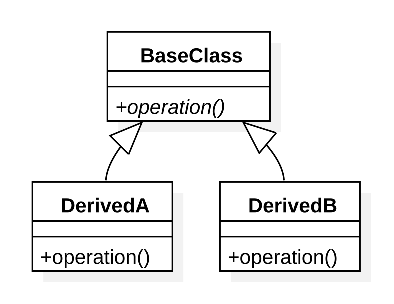
\includegraphics[width=0.35\linewidth]{images/illustrative/runtime polymorphism.eps}
    \caption{Пример реализации динамического полиморфизма виртуального метода на диаграмме классов}
    \label{fig:cpp-runtime-polymorphism-example}
\end{figure}

Важно заметить, что в C++ не включены лексические средства для
описания интерфейсов, как это сделано в таких языках как Java
или C\#. В C++ интерфейс, как элемент неявно включён в виртуальный
класс. В то же время, в тех случаях, когда по каким-то причинам,
интерфейс всё же должен быть обозначен в коде программ сам по себе,
прибегают к идиоматическому представлению посредством объявления абстрактного класса
(или структуры) не содержащего атрибуты, с одними чисто-абстрактными
методами. В этом случае, структура типов выглядит подобно примеру
изображённому на рисунке~\ref{fig:cpp-runtime-polymorphism-example-w-iface},
где интерфейс \texttt{BaseClass} вынесен в отдельный тип
данных~\texttt{BaseClassIFace} обобщающий класс~\texttt{BaseClass},
наследники которого уже и реализуют интерфейс.

\begin{figure}
    \centering
    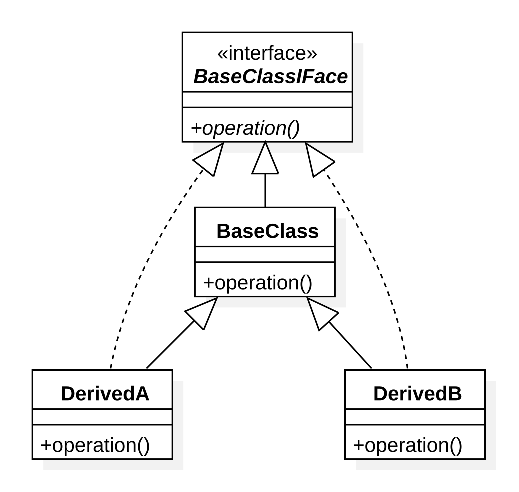
\includegraphics[width=0.5\linewidth]{images/illustrative/runtime polymorphism w iface.eps}
    \caption{Пример реализации динамического полиморфизма в C++ с выделенным интерфейсом на диаграмме классов}
    \label{fig:cpp-runtime-polymorphism-example-w-iface}
\end{figure}

Статический полиморфизм
разрешается на этапе компиляции, обычно через перегрузку функций
и операторов, а также шаблоны \cite{Stroustrup2013}.
Статический полиморфизм в C++ широко используется для достижения
настраиваемого поведения на этапе компиляции без накладных
расходов динамической диспетчеризации. Он реализуется
посредством т.н. traits-типов (в ряде источников -- \emph{свойства},
\emph{шаблоны свойств}), частичной или полной специализации
шаблонов, часто с применением идиомы
\acrshort{sfinae} (англ. \emph{Substitution failure Is not an error},~\cite{Vandevoorde2002-cpp-templates}) -- то есть
механизмом, позволяющим исключать неподходящие
шаблонные инстанцирования при разрешении перегрузок, реализуя,
таким образом систему \emph{классов типов}, подобную той что применяется в
некоторых функциональных языках (Scala, Haskell). Кроме
того, статический полиморфизм может быть достигнут с
помощью идиомы \acrshort{crtp}~(англ. \emph{curiously recurring template pattern},~\cite{Abrahams2005-cpp-metaprogramming}),
при котором классы наследуют шаблон, параметром которого является
сам класс-наследник, что обеспечивает разрешение виртуальной
функциональности на этапе компиляции.

Пример статического полиморфизма с использованием traits-типа
изображён на рисунке \ref{fig:cpp-static-polymorphism-example}.
В качестве полиморфной сущности рассмотрен
класс~\texttt{Subject} параметризуемый типом~\texttt{T}.
Класс~\texttt{Subject} содержит обобщённую программу, в которой
определения типов, вызов конкретных процедур или использование
определённых значений делегируется некоторому шаблонному
типу~\texttt{Traits}, параметризуемому типом~\texttt{T}, в общем
случае не обязательно определённому.
В этом случае, возможно определять полные или частичные (в т.ч.
с использованием \acrshort{sfinae}) специализации типа~\texttt{Traits<T>}
во внешних модулях программ, таким образом дополняя и обогащая
реализации обобщённых алгоритмов в~\texttt{Subject<T>}
соответствующими расширениями. На приведённом примере
инстанцирование шаблона~\texttt{Subject<float>} выводит
конкретную реализацию~\texttt{Subject} на основе информации
предоставленной~\texttt{Traits<float>}.

\begin{figure}
    \centering
    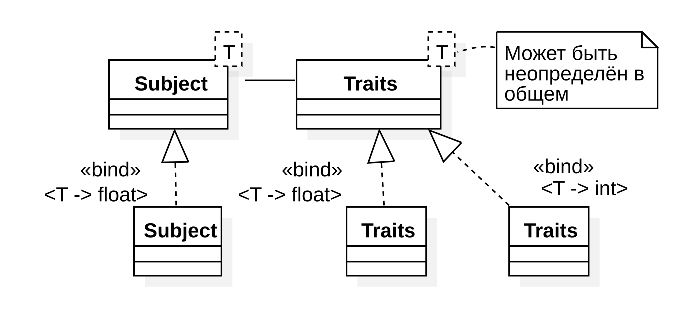
\includegraphics[width=0.7\linewidth]{images/illustrative/static-polymorphism-example.eps}
    \caption{Пример статического полиморфизма на основе шаблона свойств}
    \label{fig:cpp-static-polymorphism-example}
\end{figure}

%Хотя по очевидным причинам, статический полиморфизм эффективен
%с вычислительной точки зрения, с точки зрения практической разработки,
%важно, что реализация статического полиморфизма в C++ посредством
%идиом CRTP и SFINAE представляет собой достаточно сложные для
%сопровождения и отладки лексические конструкции. 
Хотя статический полиморфизм обладает очевидными преимуществами
с вычислительной точки зрения, его практическое применение в C++
сопряжено с определёнными трудностями. Реализация посредством идиом
\acrshort{crtp} и \acrshort{sfinae} приводит к возникновению сложных для сопровождения
и отладки лексических конструкций (грамматика
языка шаблонов вводились в C++ поверх существующего стандарта языка,
и не предусматривает соответствующей функциональности в виде
явных лексических конструкций).
Кроме того, статический полиморфизм характеризуется высокой
инфраструктурной инвазивностью.
По этим причинам,
решение о предоставлении публичным \acrshort{api} точки расширения
реализуемой посредством статического полиморфизма, должно приниматься
в рамках глобальной архитектуры приложений.
%, что делает его использование
%в качестве механизма расширения публичного
%\acrshort{API} оправданным лишь в случае, если такое решение согласовано
%с общей архитектурой системы.


%Основное внимание в последующем изложении уделено описанию обобщённых контекстов и типовых сценариев использования, которые служат основой для разработки
%соответствующих технических решений, с указанием соответствующих
%принципиальных ограничений. Целью главы является выделение конечного
%набора обобщённых решений, охватывающих потребности рассматриваемой
%области в целом и формализующих её типовые задачи, при этом
%предусматривается определение конкретных точек расширения,
%позволяющих адаптировать эти решения к специфическим условиям отдельных
%экспериментов, подсистем и этапов исследований.
Дальнейшее изложение сосредоточено на описании обобщённых контекстов и типовых сценариев использования, которые образуют основу для разработки соответствующих технических решений с фиксацией их принципиальных ограничений. Целью главы является выделение конечного набора обобщённых решений (\emph{инвариантов} системы),
охватывающих совокупность потребностей рассматриваемой области и
формализующих её характерные задачи. При этом предусматривается
определение конкретных \emph{точек расширения}, обеспечивающих адаптацию
указанных решений к специфическим условиям отдельных экспериментов,
подсистем и этапов исследований.

\section{Специфика предметной области}

С момента появления записывающей техники в области высокоэнергетических
экспериментов широкое распространение получила концепция эксперимента с
триггером~\cite{nucl-exp-methods-Grigorev1988}. В её рамках часть
детекторов выделяется в качестве триггерных,
а их сигналы обрабатываются логической функцией для принятия решения о записи
данных на основе откликов быстрых детекторов. Наличие или отсутствие сигналов
от определённого набора детекторов (составляющего лишь часть всего набора
детекторов установки и называемых \emph{триггерными детекторами}),
а также быстрая оценка физических величин
относительно заданных порогов, составляют входные параметры логического
условия. Срабатывание триггера задаёт временную точку отсчёта для
оцифровывания сигналов детекторов в некотором временном окне.
Совокупность данных записанных таким образом упорядочивается в рамках
структуры данных отдельного события. Классическим примером является
эксперимент Коуэна и Рейнеса по регистрации антинейтрино в
1954 году~\cite{cowan1956detection},
в котором основой для выделения событий взаимодействия антинейтрино с
протонами являлось фиксированная временная разница между чувствительными
элементами установки определяемая замедлением нейтронов в веществе
мишени.

Следует отметить, что понимаемый под (оцифрованным) \emph{событием}
набор данных в терминологии информационных систем не всегда строго
соответствует событию в вероятностном смысле. Хотя предполагается,
что события независимы, с определённой частотой — зависящей от
интенсивности исследуемого процесса — возможно наложение статистически
независимых событий во временных интервалах, определяемых длительностью
временного окна и инерционностью откликов детекторов. Этот эффект
естественно обусловлен физическими ограничениями, такими как время развития
электромагнитных и адронных ливней, лавинных процессов, а также
остаточной ионизацией в рабочих объёмах детекторов, сигналами от
вторичных частиц, гало пучка и т.д.

\subsection{Логический триггер}

В экспериментах с большим числом наблюдаемых каналов используется
многоуровневая триггерная система~\cite{nucl-exp-methods-Grigorev1988},
включающая триггеры различных
уровней (например, \emph{L1} — <<\emph{Level 1}>>, \emph{L2} и
последующие). Низкоуровневые аппаратные триггеры реализуются с
использованием аналоговых и дифференциальных схем, а также электроники
с наносекундным и пикосекундным временным разрешением. Их основная
задача --- обеспечить быстрый, предварительный отбор событий по сигналам
детекторов, подавляя таким образом комбинаторный фон сигналов от реакций,
не представляющих физического интереса.

Триггеры более высоких уровней, как правило, реализуются на менее
быстродействующей, но более гибкой цифровой компонетной базе:
на программируемых
логических интегральных схемах (\acrshort{fpga}), а также в виде
программных триггеров, выполняемых на
универсальных процессорах.

%То как именно соотносится программное представление события
%и его программная модель (цифровой образ) --- очень важный вопрос
%архитектуры \acrshort{sw} физического эксперимента.

Особое значение имеет то, каким образом соотносится информация о
событии и его цифровая модель в смысле логического соответствия
статически-типизированным данным. Этот аспект представляет собой ключевой вопрос
архитектуры программного обеспечения физического эксперимента, и его решение
можно можно сформулировать в виде различного рода формальных схем или
диаграмм.

%К примеру, проблема временного перекрытия событий, обусловленного
% чисто статистическими эффектами (для постоянной средней интенсивности
% временные интервалы между событиями подчиняются экспоненциальному распределению).
% В простейшем случае \acrshort{sw} может быть спроектировано таким образом, чтобы после записи событий
% от L1-триггера, события идентифицированные как pile-up отбраковывались и не учитывались в анализе. Такой подход
% не требует разрешать вклады от отдельных статистически-независимых событий. В тех случаях, когда
% интенсивность исследуемой реакции достаточно велика,
% чтобы результат измерений удовлетворял заданному порогу
% статистической значимости, а аппаратура подвержена влиянию
% сложных эффектов приводящих к трудноразрешимым
% неоднозначностям, такой подход оправдан и приводит к
% сравнительно простой архитектуре \acrshort{sw}:
% <<одна сигнатура --- одно событие>>.
% Более сложные случаи подразумевают присутствие в отклике детекторов информации о нескольких событиях, в том числе не обязательно сигнальных. В этом случае программная модель события уже не обязательно соответствует единственному исследуемому событию, хотя для упрощения задач анализа может быть целесообразно сохранить их логическую связь в виде выделенного программного представления.

К примеру, одной из характерных проблем в регистрационных системах является
временное перекрытие событий, обусловленное статистическим
эффектом~(частотной перегрузке, перекрытием
сигналов, англ. \emph{pile-up}): при постоянной средней интенсивности временные
интервалы между событиями подчиняются экспоненциальному
распределению. На практике это означает, что в пределах одного
временного окна могут присутствовать отклики
от нескольких независимых событий.

В простейшем случае программное обеспечение может быть организовано
таким образом, чтобы после записи события, фильтрация, выполняемая при
анализе, отбраковывала записи, идентифицированные как результат
наложения событий, исключая их из дальнейшего анализа.
Такой подход не требует разрешения вклада от индивидуальных
статистически независимых событий и, при определённых условиях, оказывается
вполне обоснованным:
\begin{itemize}
    \item Если интенсивность исследуемого процесса достаточно высока для
    достижения необходимой статистической значимости результатов.
    \item Или если влияние аппаратурных эффектов приводит к возникновению
    неоднозначностей в интерпретации сигналов, которые затруднительно, или
    невозможно устранить алгоритмически.
\end{itemize}

В подобных случаях достигается относительная простота архитектуры \acrshort{sw},
основанной на принципе: <<одна сигнатура — одно событие>>.
В этом случае отношение между оцифрованным сигналом от детектора и
экземпляром события выглядит как простая ассоциация, изображённая на
рисунке~\ref{fig:simple-hit-event}, в котором тип данных~\texttt{Hit}
содержит информацию об отдельных откликах детектора, и его экземпляры
включены посредством композиции в экземпляр события представленный
типом данных~\texttt{Event} выражающим информацию об отдельном событии.

\begin{figure}[ht!]
    \centering
    
\includegraphics[width=0.25\linewidth]{images/illustrative/simple-event-struct.eps}
    \caption{Простейшая модель отклика детектора в событии}
    \label{fig:simple-hit-event}
\end{figure}

Более сложные сценарии предполагают, что отклик детекторной системы
может содержать информацию от нескольких перекрывающихся событий, включая
как сигнальные, так и обусловленные фоном. В таких условиях программная
модель записанного события инициированного триггерной системой уже не
обязательно соответствует одному акту взаимодействия.
Для упрощения дальнейшего анализа целесообразно
сохранять логическую связность таких данных в виде единого программного
представления (записи) о записи события по триггеру, при этом разделяя вклады
от различных первичных взаимодействий. Вариант реализации приведён на
рисунке~\ref{fig:complex-hit-event}, на котором тип данных события~\texttt{Event}
включает через композицию экземпляры типов данных с информацией об отдельных
откликах, объединяемых посредством агрегации в типе~\texttt{TimeCluster}.
Последний можно представить и в виде класса ассоциации в тех случаях, когда
по каким-то причинам необходима нормализация коллекции~(например, хранение в реляционной~\acrshort{db}).

\begin{figure}[ht!]
    \centering
    %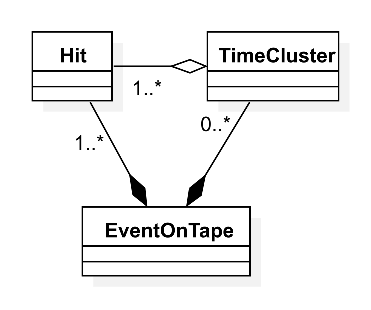
\includegraphics[width=0.33\linewidth]{imgs.view/illustrative/complex-event.eps}
    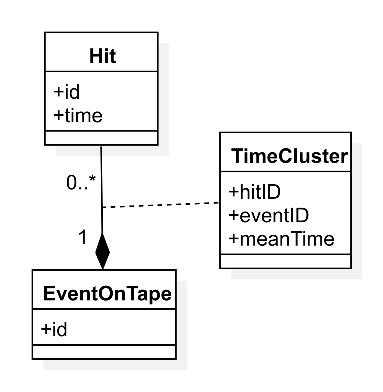
\includegraphics[width=0.33\linewidth]{images/illustrative/hit-assoc.eps}
    \caption{Модель события с разделением откликов во времени с классом ассоциации}
    \label{fig:complex-hit-event}
\end{figure}

В тех случаях, когда разделение откликов во времени неоднозначно, и конкурентные
гипотезы должны рассматриваться одновременно, может потребоваться введение
дополнительных классов ассоциации. На рисунке~\ref{fig:more-complex-hit-event}
вводится дополнительный тип данных~\texttt{Event} агрегирующий информацию о
конкурирующих гипотезах, выраженных посредством различной группировки
временных кластеров.

\begin{figure}[ht!]
    \centering
    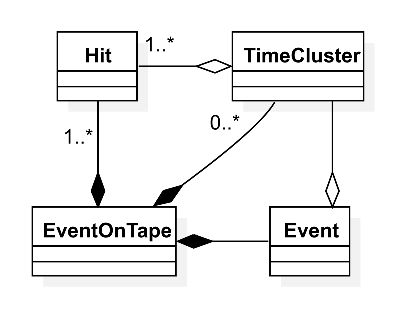
\includegraphics[width=0.33\linewidth]{images/illustrative/more-complex-event.eps}
    \caption{Модель события с разделением откликов во времени представляющая конкурирующие гипотезы}
    \label{fig:more-complex-hit-event}
\end{figure}

Описанные варианты организации модели события и его частей часто встречаются в
иерархии данных при обработке данных физического эксперимента. Другими примерами
могут быть треки частиц, образованные различными комбинациями пространственных
показаний трековых детекторов, амплитуды ячеистых калориметров образующие
пространственные кластеры, сигналы от многослойных трековых детекторов и т.д.
Различные способы представления составных типов данных включают кортежи,
таблицы, реляционных таблицы, структуры и классы, соответствующие выбранным
языковым средам.

\subsection{Модель события}

Среди доступных способов описать модель события в компьютерной программе выделим
следующие, как нашедшие наиболее широкое применение в практике организации
научного \acrshort{sw}:

\begin{itemize}
    \item \emph{Табличная модель}
    %описывает результаты
    %измерения отдельного события в виде кортежа~(строки)
    %%вещественных чисел~$v_i \in \mathbb{R}$
    %в котором
    %информация о принадлежности измерения $v_i$ кодируется
    %индексом~(колонкой)~$i$.
    представляет результаты измерений, относящихся к отдельному физическому событию, в виде
    кортежа (строки), компоненты которого интерпретируются как числовые значения,
    соответствующие различным характеристикам события. Идентификация каждого значения
    $v_i$ осуществляется посредством его позиции или имени соответствующего
    столбца $i$, что позволяет явно связать измеряемую величину с её смысловым
    назначением (позиционная семантика).
    \item \emph{Реляционная модель}
    %описывает событие в
    %виде наборов строк из взаимосвязанных таблиц между
    %которыми определены реляционные отношения. Для
    %эффективного использования этого подхода необходимо
    %соответствие модели т.н. \emph{нормальным формам},
    %описанным в теории реляционных таблиц.
    описывает событие как совокупность записей, организованных
    в виде взаимосвязанных таблиц, между которыми заданы формальные
    реляционные зависимости. Эффективное применение данного подхода требует
    приведения представления модели к формам,
    обеспечивающим согласованность и непротиворечивость представления,
    что формализуется в рамках т.н. \emph{нормальных форм} реляционной теории.
    \item \emph{Структурная модель} рассматривается в рамках
    т.н. структурированного %(<<\emph{structured programming}>>\footnote{в
    %ряде отечественных источников --- \emph{структурированного}})
    программирования и вводит иерархическое представление
    поверх реляционной модели посредством специализированных
    выразительных средств целевой среды. Для эффективной
    работы при таком описании не является обязательным
    нормализация отношений модели.
    \item \emph{Объектная модель} исторически рассматривается как
    расширение структурной модели в рамках парадигмы объектно-ориентированного
    программирования (\acrshort{oop}), которая дополняется средствами
    %инкапсуляции, наследования и полиморфизма,
    средствами описания динамического поведения экземпляров
    позволяя задать как структуру,
    так и поведение элементов данных. В рамках этой модели
    физические объекты или события представляются экземплярами
    классов с внутренним состоянием и набором методов взаимодействия.
\end{itemize}

%Заметим, что хотя перечисленные способы не являются
%взаимоисключающими и во многих случаях допускают
%автоматизированную конверсию из одного представления в
%друге (при обязательной рефлексивности данных).
Следует отметить, что указанные модели представления данных не являются
взаимоисключающими и, при условии наличия полной рефлексивной информации
о структуре и семантике данных, допускают автоматизированное преобразование
одной формы в другую.

%Табличный способ и описание посредством реляционной модели
%крайне эффективны при проведении анализа на
%высоком уровне, поскольку современные программные средства
%(такие как \emph{R}, \emph{pandas} (Python), \emph{Matlab} или  % TODO: ссылка
%различные \acrshort{dbms}) предоставляют широкий набор различных агрегатных функций
%для выполнения наиболее частых операций анализа: подсчёта
%моментов распределений над выборками, свёртки, объединения
%таблиц и т.д. Парадигмально, программы на функциональных
%языках оперирующих с табличными данными и списками (\emph{R},
%\emph{Lisp}, \emph{Haskell}) выразительны, лаконичны,
%часто превосходят императивные языки по быстродействию
%за счёт оптимизации на чистых функциях.
%Однако, с точки зрения универсальности
%представления, табличный вид имеет существенный недостаток
%при определении разрежённых~(\emph{sparsed}) данных.
Табличный способ представления данных, а также его формализация
посредством реляционной модели, демонстрируют высокую эффективность
при выполнении статистическог анализа, что полезно было бы использовать
и для физических задач. Современные высокоуровневые
программные средства, такие
как язык и программное окружение \emph{R},
библиотека \emph{pandas} (Python), язык и программное
окружение \emph{Matlab}, а также различные системы управления
базами данных (\acrshort{dbms}), --- предоставляют обширный
набор агрегатных операций, охватывающий типичные задачи: вычисление
статистических моментов по выборкам, выполнение свёрток, объединение
таблиц и прочее.

%С парадигмальной точки зрения, программирование на функциональных языках, ориентированных на обработку табличных структур и списков (\emph{R}, \emph{Lisp}, \emph{Haskell}), отличается высокой выразительностью и лаконичностью. В ряде случаев такие языки демонстрируют более высокую производительность по сравнению с императивными подходами, благодаря эффективной оптимизации чистых функций,
%оптимизации на хвостовой рекурсии, локализации на стеке.

Тем не менее в контексте универсальности представления,
табличные структуры обладают существенными ограничениями,
в основном проявляющимися при работе с разрежёнными данными.

%Реляционный вид, хотя и лишён такого недостатка, неудобен при работе
%в императивных языковых средах. Это неудобство
%является определяющим для задач анализа данных физического эксперимента,
%поскольку соответствующая архитектура должна в первую очередь
%отвечать приоритету низкой сложности и динамики прототипов программной
%реализации алгоритмов реконструкции. 
Несмотря на принципиальную возможность учесть разрежённость данных в
рамках реляционного подхода, он малопригоден для практического
использования в императивных языковых средах из-за лексической громоздкости
соответствующих запросов, необходимости всякий раз формулировать условия
объединения. Это обстоятельство является критически важным в контексте
задач анализа данных физического эксперимента, где архитектура
программного обеспечения должна, прежде всего, обеспечивать
низкую сложность и высокую гибкость при прототипировании алгоритмов
реконструкции.
%Функциональное программирование
%и связанное с ним семейство выразительных средств недоступно
%широкому кругу технических специалистов работающих в
%экспериментальной физике и \acrshort{hep}. Так, например,
%специализированный язык для статистических расчётов \emph{R},
%не взирая на популярность в индустрии и у специалистов профессионально занятых статистикой,
%нашёл лишь умеренную популярность среди аналитиков в \acrshort{hep}.

%Основная функция реляционных \acrshort{dbms} --- быстрый поиск, вставка и
%удаление записей в таблицах, оптимизированные для случайного
%доступа. Программная архитектура таких приложений
%выстраивается под работу с индивидуальными записями.
Основное назначение реляционных систем управления базами данных
(\acrshort{dbms}) заключается в обеспечении высокоэффективного поиска, вставки
и удаления записей в таблицах, оптимизированных под случайный доступ
к данным. Соответственно, программная архитектура подобных приложений
ориентирована на работу с отдельными записями.
Напротив, в рассматриваемых сценариях использования чаще всего требуется потоковое
применение алгоритма над большой последовательностью записей.
Для такой задачи оптимизация должна производиться под
последовательную вычитку. Вставка записей в таблицу
на этапе реконструкции производится последовательно, а удаление
записей бывает нужно лишь в отдельных случаях.

Значительно более существенную проблему представляет сложная
иерархия данных физического события: группирование по типам
данных, двунаправленные ассоциации, отношения <<многие ко многим>>
и необходимость частых переходов между уровнями этой иерархии
приводят к большому количеству операций соединения (с точки зрения
реляционной алгебры), созданию промежуточных таблиц и существенно
затрудняют разработку алгоритмов.

Таким образом, применение реляционных таблиц в качестве основного средства
хранения и доступа к данным физического эксперимента не отвечает
основным вариантам использования модели события. Однако, следует
заметить, что в рамках предмета автоматизации физического эксперимента в
целом, существует большое количество сценариев которым
реляционные \acrshort{dbms} отвечают вполне: сопровождение калибровочных данных,
хранение метаданных, журналирование и телеметрия оборудования,
синхронизация пакетных вычислений и т.д.

В то же время, структурная модель вполне отвечает приоритету
простоты и доступности. В рамках такого
описания производят логическое разделение данных события на
семантические группы соответствующие понятиям <<событие>>,
<<кластер>>, <<трек>> и т.д. В рамках структурного
программирования этим понятиям ставят в соответствие
типы данных (посредством специализированных выразительных
средств --- объявляя типы составные данных, таблицы, кортежи).
Такая декомпозиция данных события
отвечает естественным категориям описания алгоритмов, и позволяет
производить разработку прототипов \acrshort{sw} прикладным специалистам.
%за счёт развитого набора сопутствующих выразительных средств
%для выборки и адресации.

Расширением структурного программирования является \acrshort{oop}, вводящее
дополнительные выразительные средства для описания динамического
поведения типов данных. Это расширяет понятие структуры данных
посредством классов, предоставляя таким образом
возможность описывать программу в виде совокупности взаимодействующих
структур данных с инкапсулированным состоянием и полиморфным
поведением.

%Следует подчеркнуть, что в рамках объектно-ориентированного подхода,
%для описания модели события, реализация поведения может относиться
%как к инфраструктуре приложений, так и к их предметному кругу. Например,
%при рассмотрении координатной метке в трековом детекторе, афинные
%преобразования координат могут быть реализованы в объектной модели
%события, что приводит к необходимости описывать согласование связанных
%состояний внутри класса координатной метки (наборы локальных и глобальных
%координат). Информационная избыточность порождённая таким образом,
%будет нуждаться в дополнительных уровнях абстракции, инкапсуляции,
%перенаправления и контроля, что оказывает существенное влияние на
%последующую архитектуру приложений для обработки. Другими подобными
%примерами могут быть любые преобразования индуцированные внешней логикой:
%применение калибровок, нормировки, фурье-преобразования и т.д.
%
%Таким образом, второй важный выбор, который необходимо сделать
%относительно объектной модели: допускается ли избыточность данных в
%модели?

В контексте объектно-ориентированного моделирования,
реализация поведения в методах классов, описывающих структуру события,
может быть отнесена к разным уровням ответственности:

\begin{itemize}
    \item \emph{Инфраструктурные аспекты реализации}, предполагающие
    осознанное ослабление изоляции классов с целью упрощения их интеграции
    в алгоритмы. К этой категории относится управление динамической памятью
    и журналирование (в простейшем случае --- стандартные потоки вывода).
    \item \emph{Алгоритмы вспомогательного характера}, выполняемые
    в рамках чётко ограниченных и изолируемых операций, таких как кодирование
    и хеширование ключей коллекций, вставка и удаление элементов.
    \item \emph{Предметно-ориентированные вычисления}, непосредственно
    связанные с логикой физического анализа, включая, например, расчёт
    производных величин (координатные преобразования, вычисление средних значений,
    вероятностные оценки по критерию Пирсона и др.).
\end{itemize}

Так, в частности, рассмотрим класс, представленный на рисунке~\ref{fig:complex-class},
описывающий координатную отметку в плоском
двухкоординатном трековом детекторе. Афинные преобразования координат
вида~$\vec{r} = f(u, v)$ могут быть инкапсулированы в объектную модель события,
как это показано на диаграмме. В этом случае между экземплярами трёх типов
данных --- двумерным и трёхмерным векторами \texttt{Vector2}, \texttt{Vector3},
а также матрицей афинных преобразований \texttt{Transform} --- устанавливается жёсткая
функциональная зависимость, которая должна быть должным образом учтена
внутри класса. Как правило, это реализуется посредством выделения
применения преобразования в приватный или защищённый метод, которые должен быть
вызван с соответствующими аргументами при опубликовании локальных координат
(методом \texttt{set\_local\_r()}) или трансформации (методом \texttt{set\_transform()}).

\begin{figure}[ht!]
    \centering
    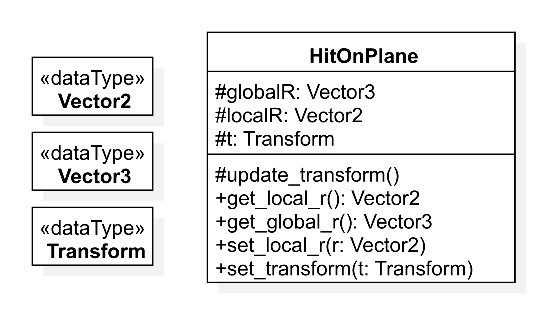
\includegraphics[width=0.45\linewidth]{images/illustrative/complex-hit-class.eps}
    \caption{Класс срабатывания координатного детектора инкапсулирующий координатное преобразование}
    \label{fig:complex-class}
\end{figure}

%В некоторых случаях предметно-ориентированные вычисления сложны, и прибегают к ленивым
%вычислениям, вводя дополнительные флаги контроля, данные кеша и транзитивные хранилища
%для того чтобы снизить потерю производительности на невостребованных элементах состояния.
В ряде случаев предметно-ориентированные вычисления обладают значительной
сложностью и сопровождаются высокой вычислительной нагрузкой. Для повышения
эффективности системы в подобных ситуациях прибегают к ленивым вычислениям,
дополнительно вводя флаги управления, кэш-память и транзитивные хранилища.
Такие меры позволяют минимизировать издержки, связанные с обработкой
невостребованных или редко используемых фрагментов состояния.

%То есть, предметно-ориентированные вычисления требуют реализации механизма согласования
%взаимосвязанных состояний внутри класса координатной метки --- таких, как локальные и
%глобальные координаты в приведённом примере. Возникающая при этом информационная избыточность
%требует введения дополнительных уровней абстракции, инкапсуляции, механизмов
%перенаправления и контроля на уровне события, что оказывает значительное влияние на
%архитектуру последующих программных компонентов обработки. К примеру, при сериализации
%(представление в виде байтовой последовательности для сохранения на диске или ленте)
%и десереализации (восстановлении) описанного в примере объекта принципиально возможно
%появление в программе экземпляра с рассогласованными локальными или глобальными координатами.
Таким образом, предметно-ориентированные вычисления требуют реализации
механизмов согласования взаимозависимых компонентов внутреннего состояния
объекта, как, например, в случае локальных и глобальных координат
отметки в трековом детекторе. Возникающая при этом информационная избыточность
предполагает введение дополнительных уровней абстракции и инкапсуляции,
а также реализацию механизмов перенаправления и контроля на уровне
объектной модели события. Эти архитектурные особенности напрямую влияют
на архитектуру и реализацию последующих компонентов программной обработки.

В частности, при \glsprepositional{serialization} (то есть представлении объекта в виде
последовательности байтов для долговременного хранения на внешних носителях)
и последующей \glsprepositional{deserialization} возможно восстановление экземпляра объекта
в рассогласованном состоянии, например, при несовпадении локальных и
глобальных координат вследствие пропуска шагов вычисления или инициализации.

%К аналогичным операциям относятся и другие преобразования на предметно-специфичном уровне
%ответственности, вызванные внешней логикой обработки, включая применение калибровок,
%масштабных преобразований, Фурье-преобразований и т.п.
Аналогичная проблематика возникает и при выполнении других
предметно-специфичных преобразований, инициированных внешними процедурами
обработки, включая применение калибровок, масштабных преобразований,
а также, например, преобразования Фурье и прочие формы предобработки и
согласования представлений.

%Таким образом, (вторым) принципиальным решением при проектировании объектной модели является вопрос,
%насколько \emph{допустима избыточность данных внутри самой модели и как должно быть
%реализовано согласование зависимых элементов}.
В этой связи, одним из принципиальных вопросов при проектировании объектной
модели является определение допустимого уровня избыточности данных
внутри структуры события и согласованной с ним стратегии
согласования зависимых элементов состояния. Примером наименее избыточных
структур данных могут быть старшие нормальные формы реляционной модели.

%Следует заметить, что архитектура претендующая на высокий уровень общности, не зависящий от конкретного
%эксперимента, не может включать в модель события предметно-ориентированные вычисления ввиду
%многочисленности и противоречивости сценариев использования, а вместо этого должна предоставить
%инфраструктуру в которой определение таких элементов поведения реализуется наиболее упрощено.
Следует подчеркнуть, что архитектура, претендующая на высокий уровень
универсальности и независимости от предметной специфики эксперимента, не может
включать в поведенческое ядро модели события реализацию предметно-ориентированных
вычислений ввиду многочисленности и противоречивости сценариев использования.
Вместо этого она должна предоставлять инфраструктуру, обеспечивающую
максимально простое и декларативное задание соответствующего поведения
в рамках внешней логики прикладного уровня.

Реализацию такого подхода целесообразно осуществить при помощи техник
\glsgenitive{metaprogramming}, опирающихся на интроспективную информацию
о модели события для генерации \acrshort{api}, которые затем также
реализуются пользовательскими алгоритмами предметно-ориентированных
вычислений.

Такой подход органично согласуется с предложенной ранее гибридной
методологией разработки ПО, отвечая второму и третьему этапам, в рамках
которых для взаимодействующих алгоритмов фиксируются структурные и
поведенческие аспекты системы.

%В заключении раздела следует заметить, что приведённые рассуждения
%в ограниченной мере справедливы и для т.н. безтриггерных экспериментов.
%В таких экспериментальных установках данные, как правило, обладают той
%или иной степенью гранулярности, обусловленной обычно техническими
%ограничениями. Часто, роль <<события на триггере>> играют временные
%окна (кадры) от потоковых источников данных, которые тем или иным образом
%соотносятся на различных уровнях предобработки (включая циклическую
%буферизацию, различные техники отбора, отыскания корелляций и т.д.),
%прежде чем попасть в персистентные хранилища. Помимо того, что в таких
%системах алгоритмическая насыщенность построения модели события может
%потребовать большей осторожности, чем процедуры реконструкция события,
%попытка построить обобщённую архитектуру предусматривающую работу с данными
%безтриггерного эксперимента обязательно потребует включение в рассмотрение
%систем отбора реализованных на вычислительных платформах различных уровней,
%что существенно увеличит набор вариантов использования системы и её сложность.
В завершение раздела следует отметить, что изложенные выше рассуждения в
определённой степени применимы и к так называемым бестриггерным
экспериментам. В подобных установках исходные данные, как правило,
обладают определённой степенью гранулярности, обусловленной
техническими ограничениями детекторов и средств сбора
информации. В них роль событий, зафиксированных триггером
выполняют временные окна (кадры), формируемые потоковыми источниками
данных и соотносимые между собой на различных этапах предварительной
обработки. Эти этапы могут включать циклическую буферизацию,
процедуры быстрого отбора (например, Фурье и вейвлет-преобразования, поиск по
КД-деревьям), алгоритмы выявления корреляций и другие методы
обработки, предшествующие записи данных в персистентные хранилища.

В контексте данной работы важно, что в таких системах построение
модели события часто сопряжено с более высокой алгоритмической сложностью,
чем в традиционных процедурах реконструкции. Разработка универсальной
архитектуры, способной обрабатывать данные бестриггерных
экспериментов, требует учёта особенностей систем отбора
данных, реализуемых на различных уровнях вычислительной инфраструктуры.
%Это, в свою очередь, существенно расширяет пространство вариантов
%использования программного комплекса и повышает общую сложность
%проектируемой системы.

\section{Сценарии использования}

Выделение сценарных контекстов использования является общим для методологий
разработки \acrshort{fdd} и \acrshort{ddd} и не зависит от конкретного
эксперимента, в то время
как набор конкретных сценариев использования может различаться от
эксперимента к эксперименту.

В этом разделе кратко описаны основные варианты использования программного
обеспечения в экспериментах \acrshort{hep}. Систематизация сценариев
производится в соответствии со следующей (индуктивной) логикой:
\begin{enumerate}
    \item На основе специфики данных выделяются основные ограничения,
    общие для работы с данными в целом, справедливые для всех
    рассматриваемых контекстов использования.
    \item На основе основных этапов жизненного цикла экспериментальных
    данных, выделяются контексты использования.
    \item В рамках перечисленных и ограниченных контекстов, выделяются
    отдельные сценарии использования.
\end{enumerate}

Сценарий использования может представлять собой отдельный модуль,
конкретную численную процедуру, функцию или класс. С точки зрения
обобщённого программирования, важно установить сходства и различия
между одним и тем же сценарием в рамках различных контекстов
использования с тем, чтобы предусмотреть набор точек расширения.

\subsection{Ограничения сценарных контекстов}

В рамках предметной области справедлива следующая специфика данных:

\begin{itemize}
    \item Для анализа редких событий и снижения неопределённости результатов,
    анализ производится на статистике достаточно большого объёма (от
    десятков и сотен терабайт), что не позволяет или существенно затрудняет
    индексирование данных в оперативной памяти вычислительных узлов и
    предъявляет высокие требования к быстродействию программ.
    \item Отдельные (с точки зрения триггерной логики) события в массиве
    данных традиционно рассматриваются как независимые. Это
    позволяет производить операции над отдельными событиями размещёнными в
    оперативной памяти целиком.
    \item Получение выборочной совокупности в анализе опирается зачастую на
    достаточно сложные критерии, включающие расчёты численными методами и
    различные агрегатные алгоритмы, которые затруднительно формулировать
    на языках запросов к реляционным таблицам.
    \item Сценарии обработки как правило формулируются в виде императивных
    программ с большим количеством циклов, ветвлений, внешних коэффициентов,
    запросов из третьих источников. Транзакционный цикл характерный для
    реляционных \acrshort{dbms} избыточен для рядовых сценариев
    обработки или анализа.
\end{itemize}

%В результате, в \acrshort{hep} к настоящему времени реляционные таблицы как основной
%носитель данных не применяется, или применяется крайне ограниченно.
Основным способом представления данных являются упрощённые структуры
типа \texttt{NTuple} или \texttt{TTree}~\cite{ROOT-framework}, представляющие
собой строковые таблицы, со сжатием, буферизацией и оптимизацией для
последовательного доступа (\emph{scan}, последовательный перебор) как основного
способа доступа к данным. Такая модель обусловлена
как структурой данных -- иерархически организованных, но при этом слабо
нормализованных, так и необходимостью применения сложных алгоритмов для
отбора записей в таблицах (событий, информации об отдельных срабатываниях,
физических кластеров, треков частиц). Модель сканирования предоставляет
линейную, предсказуемую модель доступа, легко поддающуюся параллелизации,
в общем не требует встраивания дополнительных индексов,
обеспечивает хорошую переносимость между различными платформами. Кроме того,
для реализации произвольного доступа, модель последовательной вычитки можно
дополнить внешними метаданными, не затрагивая физическое размещение
основных данных в тех случаях, когда формат сам по себе допускает произвольны
доступ.

С этой точки зрения, архитектурное решение относительно основной модели
доступа к данным на раннем этапе заключается в выборе между строковым и
колончатым представлением таблиц, поскольку именно связанные с физической
моделью данных архитектурные  ограничения наиболее трудно преодолеть
впоследствии.

Требования к быстродействию программ актуальны при работе с большими
объёмами данных, типичными для \acrshort{hep}. В то же время, язык используемый для разработки программ должен обеспечивать достаточно широкий набор выразительных
средств, не требующий высокой квалификации для разработки и сопровождения.
Достаточно хорошо этому требованию отвечает семейство языков C. Сопутствующий
набор библиотек предоставляет надёжные реализации численных методов и
широкий набор общих алгоритмов для составления выразительных программ в
императивной логике.

С учётом изложенных особенностей, сформулируем основные черты и ограничения
проектируемого программного комплекса:
\begin{itemize}
    \item Обработка отдельных событий производится в оперативной памяти,
    при этом хранение всего объёма данных возможно в том числе и на
    распределённых хранилищах большого объёма.
    \item Последовательный доступ к потоковым данным из принципиально
    неограниченного источника (потока) используется как основная модель
    доступа к данным. При этом запись соответствующая событию декодируется
    целиком (последовательный доступ для строковых данных как основная
    модель доступа к данным).
    \item C и C++ используются в качестве основных языков реализации
    программ реконструкции.
\end{itemize}

В рамках предложенной методологии разработки, для стратификации вариантов
использования программного окружения для реконструкции событий, необходимо
произвести выделение общих сценарных контекстов. Для этого, рассмотрим
основные этапы жизненного цикла эксперимента с точки зрения применения
прикладного \acrshort{sw}:
\begin{itemize}
    \item \emph{Предварительное численное моделирование эксперимента}. В
    современном физическом эксперименте, моделирование применяется
    при выборе постановки эксперимента для измерения конкретных
    каналов реакций, на этапе разработки технического предложения.
    Оценивается принципиальная возможность проведения измерений с учётом
    выхода реакции, светимости отдельных каналов, геометрии и разрешения
    детекторов. Данный этап в ограниченной форме подразумевает
    реконструкцию событий или применение отдельных алгоритмов.
    \item \emph{Тестирование отдельных детекторов и детекторных сборок}
    (англ. <<research and development>>, R\&D). В рамках этого этапа
    производится тестирование и отладка отдельных конструктивных
    компонент установки: модулей калориметров, трекера. Ограниченно
    применяются (и тестируются) алгоритмы, которые впоследствии будут
    включены в общую реконструкцию событий.
    \item \emph{Набор данных}. Сеансы набора данных обычно упорядочены
    в определённых хронологических интервалах, подразумевающих
    определённое постоянство условий измерения. С этой целью
    необходимо применение развитых средств наблюдения за установкой,
    оперативной диагностики её подсистем.
    \item \emph{Калибровка детекторов}. Может производиться как
    на основе выделенных сеансов набора данных, так и во время
    набора физических данных. Часто включает информацию полученную
    во время R\&D-фазы. Обычно подразумевает реконструкцию и анализ
    в ограниченной форме.
    \item \emph{Анализ физических событий}. На данном этапе необходимо
    наиболее полное знание об условиях измерения, доступ ко всей
    накопленной статистике с целью наиболее полной и достоверной
    реконструкции отдельных физических величин и физических событий
    в целом. Выполняется с привлечением высокопроизводительных
    средств, в окружениях пакетного счёта (\acrshort{htc}, \acrshort{hpc}).
    Результатом измерений являются конкретные значения физических величин,
    функции плотности вероятности, их интегральные оценки,
    доверительные интервалы, результаты проверки статистических гипотез.
\end{itemize}

Важно, что моделирование эксперимента, вообще говоря, должно в конечном
итоге воспроизводить реальные данные, и методически не должно обладать
значимым количеством специфических особенностей и свойств, отличающих
задачи обработки результатов моделирования от задач анализа данных.

На основе этапов жизненного цикла, рассмотрим основные сценарные контексты
в модели потоковой обработки.

\subsection{Анализ физических величин и событий}

Реконструкция физических величин производится на основе откликов детекторов
с использованием предварительно полученных калибровочных
данных, а также различной информации, отражающей известные
характеристики экспериментальных условий, справочной информации и
распределений известных из первых принципов.

Программные интерфейсы соответствующих вычислительных сред, как
правило, оптимизируются с расчётом на данный сценарный контекст, как
наиболее приоритетный, поскольку именно он характеризуется наибольшей
алгоритмической сложностью в рамках всей проблематики анализа данных
физического эксперимента.

В типичном случае сценарий реконструкции предполагает задание
алгоритма, осуществляющего преобразование входных данных, частично
или полностью содержащих информацию о событии и представленную в
терминах объектной модели, в выходной набор данных в том же формате.
Рассмотрим ряд наиболее характерных задач реконструкции событий:

\begin{itemize}
    %\item Выделение зарядовых кластеров на основе набора
    %откликов многопроволочных или микропаттерных газоразрядных
    %детекторов. Принципиально, может быть произведено на основании
    %одной лишь информации из модели события, без использования калибровочных данных.
    \item Выделение зарядовых кластеров на основе откликов многопроволочных или микропаттерных газоразрядных детекторов. Такая операция может выполняться исключительно по информации, содержащейся в модели события, без привлечения калибровочных данных.
    
    %\item Формирование набора зарядовых кластеров,
    %составляющих гипотезу о треке частицы. Для корректного выполнения
    %такой задачи, как правило, необходимо привлечение информации
    %о геометрии детекторов (внешней по отношению к содержащейся в
    %модели события), позволяющей исключить с физической точки
    %зрения маловероятные или невозможные конфигурации.
    \item Формирование совокупности кластеров, составляющих гипотезу о треке частицы. Для этого обычно требуется знание геометрии установки, позволяющее исключать физически маловероятные или невозможные конфигурации.
    
    %\item Аппроксимация выбранной совокупности кластеров моделью трека.
    %В зависимости от используемого метода подгонки (фитирования) может
    %потребоваться учёт дополнительной информации: матриц
    %ковариации, зависящих от пространственного разрешения детекторов;
    %пространственной карты распределения материала внутри детектора,
    %влияющей на эффект множественного рассеяния; а также пространственной
    %карты напряжённости магнитного поля, необходимой при наличии
    %отклоняющих магнитов в спектрометре. Результатом работы
    %подобного (как правило, вычислительно-сложного) алгоритма
    %является набор параметров, характеризующих реконструированный трек
    %частицы: её заряд, массу, кинематические характеристики и ожидаемые
    %отклонения в материале активного объёма.
    \item Аппроксимация выбранных кластеров моделью трека. Здесь могут учитываться ковариационные матрицы, зависящие от разрешения детекторов, карта распределения материала (влияние множественного рассеяния) и карта магнитного поля. Результатом является набор параметров, характеризующих реконструированный трек: заряд, массу, кинематические характеристики и их ожидаемые отклонения.
    
    %\item Оценка энерговыделения от электромагнитного или адронного ливня
    %в веществе калориметра на основе откликов, регистрируемых
    %зарядово-цифровыми преобразователями. Перевод измеренной амплитуд в
    %энергетические единицы осуществляется с использованием функции
    %отклика, параметры которой определяются в процессе предварительной
    %калибровки.
    \item Оценка энерговыделения от электромагнитного или адронного ливня в калориметре по амплитудным сигналам на входах \acrshort{adc}. Перевод амплитуд в энергетические единицы осуществляется на основе функции отклика, параметры которой определяются калибровкой.
    
    %\item Формирование комбинаторных конфигураций элементов
    %модели события для последующей оценки физических гипотез и отбора
    %наиболее правдоподобных интерпретаций с применением иных
    %алгоритмов.
    \item Формирование комбинаторных конфигураций элементов события для проверки физических гипотез и отбора наиболее правдоподобных интерпретаций.
\end{itemize}

%Такие алгоритмы, как правило, допускают формулировки на различных
%уровнях общности, позволяя декомпозицию сложной многосоставной
%задачи реконструкции физического события на более простые
%логически-изолированные этапы.
Подобные алгоритмы допускают формулировку на разных уровнях общности, что позволяет декомпозировать сложную задачу реконструкции события на более простые логически-изолированные этапы. Важной их особенностью является \emph{детерминированность}: преобразование входных данных алгоритмом должно быть в точности воспроизводимым.
На наиболее общем уровне, иерархию вариантов использования в контексте анализа
данных можно свести к трём наиболее общим сценариям, изображённым на
рисунке~\ref{fig:analysis-main-usecases}: оценке функции
плотности вероятности и связанных величин, составлению выборок данных,
и сохранению выборки событий (перенаправлению потока данных).

\begin{figure}[ht!]
    \centering
    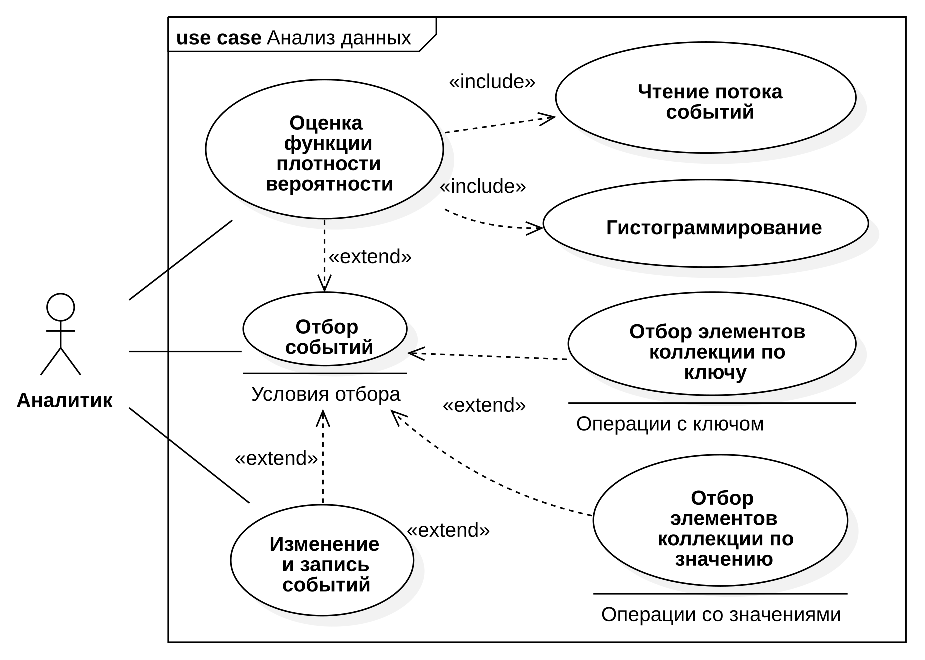
\includegraphics[width=0.85\linewidth]{images/usecases/analysis-usecase.eps}
    \caption{Диаграмма вариантов использования в сценарном контексте анализа данных}
    \label{fig:analysis-main-usecases}
\end{figure}

Для высокоуровневых сценариев отбора событий вводится точка расширения
в которой должен реализовываться отбор, в то время как логика
вычитки и обработки событий может быть реализована в обобщённой
форме. На более низком уровне, во множестве условий отбора, с технической
точки зрения необходимо различать отбор элементов коллекций по
значению и отбор по ключу, поскольку различия в реализации между этими
вариантами весьма существенны.

Главной отличительной особенностью такого контекста является требование к
\emph{детерминированности} вычисления (реконструкции) --
преобразование входных данных алгоритмом должно всегда
оставаться воспроизводимым. Иными словами, преобразование
входных данных должно быть идемпотентно.

\subsection{Сопровождение набора данных}

Другим распространённым сценарием использования программного
окружения является сопровождение эксперимента в ходе набора данных.
В данном случае речь идёт о контроле состояния детекторов и их
диагностике в режиме реального времени (онлайн-реконструкция).
Практически это реализуется посредством случайной выборки небольшой
доли событий из непрерывного потока, что позволяет получать
репрезентативную статистику в ограниченном временном окне, имеющем
фиксированную хронологическую или логическую привязку.

Ключевое отличие данного сценария от полной реконструкции заключается
в приоритете скорости обработки и устойчивости алгоритмов над
точностью и глубиной анализа. Целью становится получение быстрых,
иногда грубых оценок, достаточных для мониторинга работоспособности
установки. В этом контексте алгоритмы реконструкции реализуются в
упрощённой форме, модели заменяются правдоподобным приближением.
Для примера рассмотрим, как задачи из предыдущей группы сценариев
изменяются в рамках данного контекста:

\begin{itemize}
    \item Выделение зарядовых кластеров на выполняется без учёта
    неэффективности чувствительных элементов, рассматривается
    их упрощённая геометрия.
    \item Составление и рассмотрение треков частиц может выполняться
    на основе ограниченного набора вариантов. Например, задача поиска
    трека формулируется без учёта множественного рассеяния, с
    усреднением координат вместо комбинаторного рассмотрения для
    многослойных детекторов
    \item Модель трека аппроксимируется упрощённой функцией
    (с пропагатором прямой или винтовой линией),
    методы Рунге-Кутта не применяются для вычисления ковариации
    в магнитном поле, само поле представлено однородной аппроксимацией
    в конечном объёме
    \item Оценка энерговыделения в откликах калориметров выполняется
    на основе глобальных максимумов сигнала или интегральных сумм ,
    без учёта нелинейностей и нестационарных
    эффектов.
    \item Анализ конкурирующих гипотез может быть заменён случайным
    выбором с целью формирования усреднённой картины.
\end{itemize}

С точки зрения высокоуровневых вариантов использования, данный контекст
представляет собой подмножество контекста анализа данных,
расширенное средствами журналирования и телеметрии, как это изображено
на рисунке~\ref{fig:online-monitoring-usecases-main}.

\begin{figure}[ht!]
    \centering
    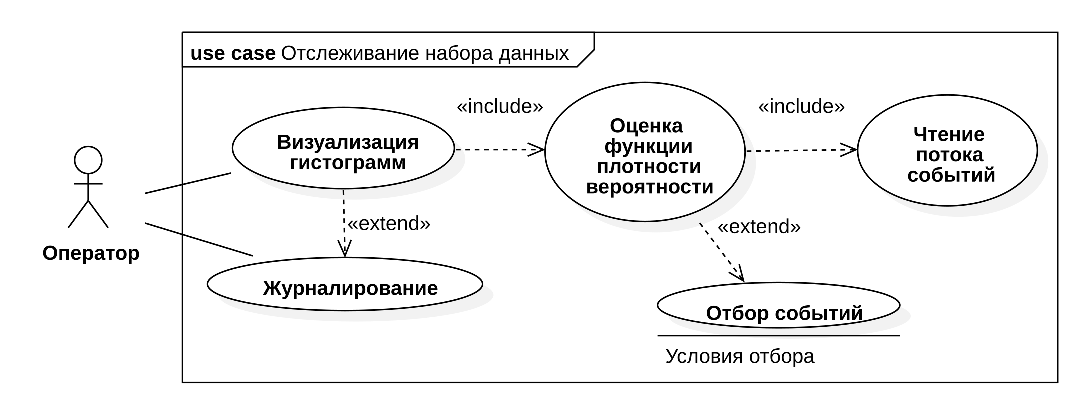
\includegraphics[width=0.95\linewidth]{images/usecases/onlineMonitoring.eps}
    \caption{Диаграмма вариантов использования в сценарном контексте сопровождения набора данных}
    \label{fig:online-monitoring-usecases-main}
\end{figure}

Требования предъявляемые к ПО в данном сценарии отличаются также
и в смысле устойчивости алгоритмов и отказоустойчивости ПО в целом.
Такое ПО предназначено для использования дежурными операторами
экспериментальной установки во время сеансов набора данных. Допустимо
снижение сценарной гибкости и статистической полноты в пользу
производительности и простоты эксплуатации. Требования
детерминированности и идемпотентности преобразований здесь
значительно слабее, чем в предыдущем контексте.

\subsection{Калибровка детекторов}

%В широком смысле калибровка детектора подразумевает отыскание аппроксимации
%\emph{функции отклика детектора}~\cite{exp-methods-Abramov1977}
%в некоторой ограниченной области. Зачастую этот сценарий требует
%получения выборки событий, отвечающей определённому критерию,
%или, напротив, -- максимального ослабления критериев отбора в
%какой-то определённой области. Так, для рассмотренных выше примеров:
В широком смысле калибровка подразумевает восстановление \emph{функции отклика детектора}~\cite{exp-methods-Abramov1977} в ограниченной области. Для этого требуется либо особая выборка событий, либо, напротив, ослабление условий отбора.
В данном контексте рассмотренные ранее примеры выражаются в следующих
сценариях:

\begin{itemize}
    \item Выделение зарядовых кластеров на микропаттерных детекторах
    обычно производится на основе характеристической диаграммы
    отношения амплитуд в области заданной
    некоторым невыпуклым многоугольником. Отыскание этого
    многоугольника представляет собой одну из задач при калибровки
    микропаттерных детекторов, для этой цели различные обрезания
    (временные и координатные) калибруемого детектора должны быть сняты.
    \item После прямых (геодезических) измерений положения детекторов проводят
    т.н. процедуру физического выравнивания (\emph{alignment})
    детекторов установки на основе реконструированной информации о
    треках, уточняя таким образом, геометрию установки, часто с точностью
    намного превышающую прямые измерения. Часто, для этого необходим
    максимально широкий пучок, засвечивающий наибольшую область
    чувствительного объёма детекторов, в широких угловых диапазонах.
    \item Задача реконструкции треков опирается на знание разрешений
    детекторов и карт их эффективности, получение которых представляет
    собой отдельную группу сценариев использования. Для этого реконструкция
    треков производится с исключённым детектором-объектом исследования.
    \item Один из вариантов калибровки калориметров состоит в отыскании
    коэффициентов пропорциональности энерговыделения регистрируемой амплитуде
    на основе известных спектров. Для этого спектры должны быть сначала
    выделены из данных, что составляет отдельную задачу анализа.
    \item Оценивание конкурирующих гипотез для калибровки нередко
    производится с ослабленными требованиями, и в этом смысле часто
    представляет собой даже более вычислительно-ёмкую задачу.
\end{itemize}

В целом, задачи калибровки детекторов во многом пересекаются с задачами
анализа, зачастую, с точки зрения сценариев использования, составляя
их подмножество, как это изображено на рисунке~\ref{fig:usecases-get-calibrations}.

\begin{figure}[ht!]
    \centering
    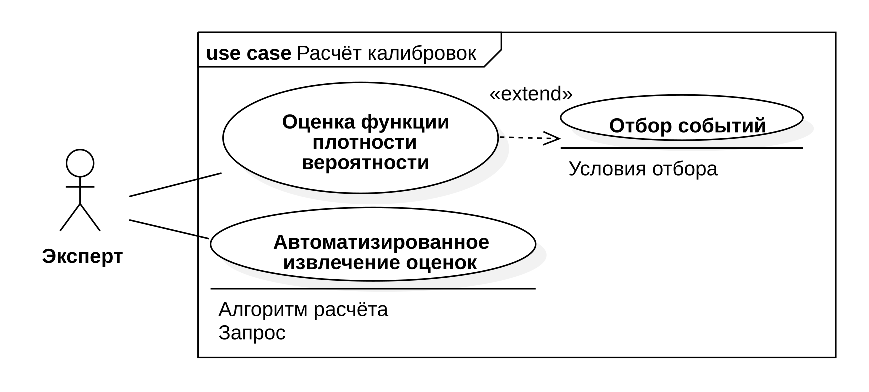
\includegraphics[width=0.75\linewidth]{images/usecases/calibration-usecase.eps}
    \caption{Диаграмма вариантов использования в сценарном контексте извлечения калибровочной информации}
    \label{fig:usecases-get-calibrations}
\end{figure}

Помимо необходимости низкоуровневого доступа к данным объектной
модели (на уровне откликов индивидуальных чувствительных элементов,
формулируемых в точке расширения <<\emph{запрос}>>),
важное прикладное значение могут иметь средства автоматизированного
извлечения информации полученной на основе функции плотности
вероятности, различных спектров и их производных значений, что
целесообразно выделить в отдельный вариант использования с соответствующей
точкой расширения (<<\emph{алгоритм расчёта}>>).

\subsection{Точки расширения на основе вариантов использования}

С точки зрения прикладного программирования, во всех перечисленных
контекстах, варианты использования имеют общие функциональные
элементы, для которых целесообразно предусмотреть обобщённые
реализации воплощающие выбранные черты архитектуры, и
предусмотреть  зависящие от конкретного эксперимента точки
расширения в которых производится реализация конкретной задачи.

\begin{itemize}
    \item  \emph{Идентификация отдельных детекторов} на различных
    логических уровнях -- от элементарных чувствительных элементов
    установки, например, ячейки калориметра, проволоки в зарядовой камере,
    стрипа в микропаттерном детекторе, до детекторных сборок, например
    модульного калориметра как целое, участка трекера вне магнитного
    поля, баррельной части установки для радиальной коллайдерной
    постановки.
    \item Работа с \emph{коллекциями} случайных величин относящихся к
    детекторам или сборкам -- итерирование, формирование выборок,
    различные свёрточные операции и агрегатные функции.
    \item Применение логических условий на случайные величины --
    логическая \emph{дискриминация} случайных величин по определённому
    признаку, выполняемая с использованием идентификаторов детекторов
    или их сборок.
    \item Функция плотности вероятности (или её аппроксимации) --
    для представления различных спектров, статистических
    перенормировок, оценки средних значений и их доверительных
    интервалов. Основным программным инструментом здесь является.
    \emph{гистограмма} (в первую очередь в смысле структуры данных,
    а не графического средства).
\end{itemize}

При этом, конкретные численные процедуры -- вроде численной аппроксимации,
решения СЛАУ, итеративной минимизации функционалов встраиваются в такую
парадигму как отдельные элементы.

Номенклатура детекторов и логическая топология определяются
конкретной установкой, иерархией её узлов и подсистем. Важно, что
объектная модель события во многом подчинена этой иерархии:
оцифрованные сигналы от отдельных чувствительных элементов
объединяются в рамках коллекций в сущности, соответствующие
физическим понятиям (зарядовый кластер, ливень в калориметре,
трек), логически отвечающие отдельным детекторам (станция трекера,
модуль калориметра, трекер). Попытка обобщить эти отношения в рамках
какой-нибудь одной системы скорее всего будет создавать больше сложностей
чем решать.

По этой причине, номенклатура детекторов и объектная модель должны
быть вынесены в точки расширения, в то время как коллекции и операции над
ними, включая логическую дискриминацию, целесообразно объединить в
рамках обобщённых алгоритмов, задающих инварианты системы.

\section{Архитектурные инварианты}

Архитектурный инвариант (англ. \emph{architectural contraint}
\cite{shaw-architecture-1996, bass-architecture}) --
это свойство программной архитектуры, которое должно
сохраняться независимо от изменений в деталях реализации или
развития системы. На основе требований сформулированных ранее,
выделим архитектурные инварианты предлагаемого решения:
\begin{itemize}
    \item Модульность -- отдельные компоненты должны
    быть изолированы так, чтобы можно было заменять
    один алгоритм реконструкции на другой без
    переписывания всей системы.
    \item Детерминированность обработки событий:
    алгоритм реконструкции при одинаковом входе
    всегда даёт одинаковый выход.
    \item Соответствие модели события и триггерной
    логики: структура данных события всегда отражает
    триггерное условие, по которому оно было записано.
    \item Потоковый доступ к данным: вся архитектура
    опирается на последовательную обработку событий.
    \item Независимость предметно-ориентированных
    вычислений от ядра системы -- логика физических
    расчётов (например, калибровки, аппроксимации
    треков) не должна входить в поведенческое ядро
    модели события, а реализуется через внешние алгоритмы
    и плагины.
    \item Иерархическая структура объектной модели
    события.
\end{itemize}

В качестве механизма обеспечивающего инвариантные свойства системы
рассматривают т.н. шаблоны (паттерны) проектирования~(\emph{architecture patterns}, \emph{software design patterns})~\cite{gof1994design-patterns}.
Шаблоны проектирования представляют собой не только типовые
решения, но и формализуют основные архитектурные ограничения
системы: они фиксируют допустимые способы взаимодействия
компонентов, ограничивают допустимые механизмы расширения и тем
самым обеспечивают сохранение инвариантов архитектуры при развитии
программного комплекса. Каждое применение шаблона проектирования можно
рассматривать как задание архитектурного инварианта: он ограничивает
пространство возможных реализаций, но гарантирует сохранение
устойчивых свойств системы — модульности, слабой связности, управляемости
расширений.
%Книга представляет собой первую попытку выделения и систематизации
%структур компьютерных программ в объектно-ориентированной парадигме,
%направленных на решение задач для которых вводится классификация по
%области применения (основные, структурные, порождающие, поведенческие),
%и типовым вариантам использования.

\subsection{Конвейерный шаблон}

Идея декомпозиции сложной процедуры на последовательность
обработчиков, каждый из которых действует независимо, выполняя
элементарную задачу над общей структурой данных, широко применяется
при организации сложных вычислительных систем достаточно давно.
В информатике, возникновение идеи и
связанной с ней терминологии можно отследить до архитектуры ранних
компьютеров (например, БЭСМ-6, \cite{smirnov-besm6}).

Классическим вариантом шаблона является
<<цепочка обязанностей>>~(\emph{chain of responsibility}).
В исполнении <<цепочки обязанностей>> прежде всего направлен на
разделение отправителей и получателей запросов в цепочке обработчиков,
архитектурный шаблон <<конвейер>> (\emph{pipes and filters})~\cite{Buschmann-patterns-vol1}
структурирует последовательную обработку данных посредством компонуемых
этапов. Хотя эти две концепции обобщают линейную последовательность
обработки, их мотивация различается:
в первом случае акцент сделан на делегировании управления потоком с
с явным указанием ответственности,
во втором важнейшим аспектом является преобразование потоковых данных.
Разделение ответственности удобно при формировании сложной и разветвлённой
логики приложений во время выполнения, и наиболее широкое применение шаблон
<<цепочка обязанностей>> нашёл при обработке событий графических
пользовательских интерфейсов, где часто применяется для динамического
связывания реакций компонентов приложения с событиями пользовательского
ввода.

Основная мотивация для использования шаблона <<конвейер>> по~\cite{Buschmann-patterns-vol1}:

\begin{itemize}
    \item Система должна позволять усовершенствования за счёт
    изменения последовательности обработчиков (на высоком уровне)
    \item Допускается повторное использование отдельных обработчиков
    в различных сценариях
    \item Несмежные обработчики не обмениваются информацией (т.е.
    передача элемента данных должна производиться от одного обработчика
    к другому, без пропусков)
    \item В системе предусмотрены различные источники входных данных,
    (файл, сетевое соединение, поток ввода).
    \item В системе должна быть предусмотрена возможность представления
    или хранения результатов различными способами
    \item Явное хранение промежуточных результатов для дальнейшей
    обработки не требуется для высокоуровневых операций
\end{itemize}

Следует также упомянуть полезное свойство <<Конвейера>>, рассматриваемое
в контексте параллельных
алгоритмов~\cite{Mattson2005-parallel-patterns, smirnov-besm6}:
когда индивидуальные обработчики действительно независимы, возможно
запускать их на параллельных системах.
% более толковое изложение (чем в книге на стр.103) у авторов на сайте:
%   https://www.cise.ufl.edu/research/ParallelPatterns/PatternLanguage/AlgorithmStructure/Pipeline.htm
% следует ли здесь подвести мотивацию к обобщённому алгоритму pipe-T?

С точки зрения реализации алгоритмов обработки, конвейерный шаблон
подразумевает реализацию обратной логики управления обработчиками.
Обработчик может инициировать прекращение обработки отдельного сообщения.
Этот результат выполнения обработчика соответствует
дискриминации физического события. Кроме того, обработчик может
инициировать остановку процесса перебора в целом, что соответствует,
например, задаче поиска события в наборе.

\subsection{Коллекции и идентификаторы}

Организация модели подразумевает все возможные типы
ассоциации: одиночное и множественное агрегирование и композицию, а
также отношение наследования между типами данных, и наследование от
коллекций. 

Рассматривая C++ в качестве основной целевой среды для генерации кода,
целесообразно воспользоваться контейнерами стандартной библиотеки
шаблонов для реализации коллекций, представляющими собой обобщённые
реализации коллекций.

Важным следствием выбора C++ в качестве основной среды является
предоставляемый всеми контейнерами стандартной библиотеки набора
выведенных типов, среди которых всегда присутствует идентификатор
играющий роль синтетического ключа (тип значения для последовательностей,
кортеж пары для карт и хэш-таблиц). Тогда индексирование коллекций
можно ограничить случаями с естественным ключом, что улучшает
читаемость прикладных программ и не приносит никаких накладных
расходов.

С алгоритмической точки зрения можно выделить три независимых качества,
которые нужно контролировать при задании типа коллекции по
естественному ключу.
\begin{itemize}
    \item Свойство упорядоченности по значениям естественного ключа
    в коллекции определяет эффективный алгоритм поиска в коллекции.
    \item Разряжённость значений ключа определяет, заполняет ли
    множество значений ключа в коллекции интервал значений без пропусков.
    \item Неоднозначность соответствия.  Во многих практических случаях
    естественный ключ должен ссылаться на множество элементов.
\end{itemize}

Поскольку каждое качество представлено в виде логического флага, определим
на их основе набор меток (англ \emph{tags}) которые впоследствии используются
метапрограммой выводящей тип коллекции на основе спецификации типа данных:
упорядоченность -- \emph{ordered}, разряжённость -- \emph{sparse} (от
англ. \emph{sparsedness}), неоднозначность -- \emph{ambig} (\emph{ambiguity}).

Три логических свойства образуют набор из восьми возможных комбинаций. Каждой
комбинации ставится в соответствие определённый контейнер стандартной
библиотеки шаблонов.

\begin{table}[ht]
    \centering
    \begin{tabular}{r|l}
        Метки & Контейнер STL \\ \hline
        \emph{ordered} & \texttt{vector} или \texttt{map} \\
        \emph{sparse} & \texttt{unordered\_map} \\
        \emph{ambig} & \texttt{unordered\_multimap} \\
        \emph{ordered, sparse} & \texttt{map} \\
        \emph{ordered, ambig}  & \texttt{multimap} \\
        \emph{sparse, ambig} & \texttt{unordered\_multimap} \\
        \emph{ordered, sparse, ambig} & \texttt{multimap}
    \end{tabular}
    \caption{Соответствие типов коллекций}
    \label{tab:placeholder}
\end{table}

Нужно заметить, что требования к типу данных ключа необходимо и достаточно
связаны с операциями которые он поддерживает. Помимо того, что
для любого ключа должна быть определена операция
сравнения ($a \ne b$), упорядоченные коллекции требуют
определения отношения порядка ($a < b$), неупорядоченные --
определения хэш-функции.

Задание коллекций через такую спецификацию меток позволяет
определить и обобщённую реализацию схему реляционных
таблиц.

\subsection{Шаблон подписки}

Калибровочные данные должны быть доступны как в процедурах
реконструкции событий, так и при онлайн-сопровождении
набора данных и при извлечении других калибровочных данных.
При этом источники информации могут быть различными:
результаты отдельных процедур анализа, внешние базы
данных, сетевые сервисы. В рамках выделенных сценариев
использования очевидна необходимость в архитектурном решении,
обеспечивающем доставку актуальных калибровочных данных
среди множества потребителей без жёсткой привязки этих
потребителей к источникам, что задаёт две точки
расширения -- тип калибровочной информации, который
целесообразно учесть через статический полиморфизм,
и поведение компонента при обновлении калибровочной информации.

Такая задача естественным образом решается в рамках архитектурного
шаблона <<издатель/подписчик>> (англ. \emph{publisher/subscriber}).
Его применение опосредует прямые зависимости между
модулями: компоненты, публикующие новые значения калибровок
(издатели), агностичны к конкретным потребителям (подписчиков).

Данное решение отвечает следующим архитектурным инвариантам:
\begin{itemize}
    \item Модульность. Издатели и подписчики инкапсулируют свои роли,
    взаимодействуя только через контракт интерфейса, что облегчает
    замену или расширение отдельных модулей.
    \item Поддержка потоковой модели обработки данных.
    Калибровочная информация распространяется синхронно, при получении
    события с определённым хронологическим идентификатором и
    не нарушает последовательную логику обработки потока
    событий, не нарушая детерминированности самих алгоритмов
    реконструкции.
    \item Гибкость точек расширения. Подписка на калибровочные
    данные может осуществляться произвольными модулями, включая
    вновь разработанные алгоритмы, без изменения ядра системы.
    \item Независимость предметно-ориентированных вычислений от
    ядра. Ядро системы агностично к конкретной логике обработки
    калибровок.
    \item Стандартизированные интерфейсы данных. События публикации
    калибровочных параметров унифицированы.
\end{itemize}

Шаблон отвечает следующим сценариям:
\begin{itemize}
    \item Источник получающий событие с хронологической меткой
    вызывает каскадное обновление всех алгоритмов реконструкции,
    подписанных на определённый тип данных.
    \item В ходе набора данных подписчики имеют актуальные
    калибровки без необходимости ручной синхронизации.
    \item Специализированные процедуры анализа могут использовать
    калибровки, подписываясь на выделенные каналы
    публикации (реализована возможность пользовательского
    переопределения калибровочных данных для подмножества компонент).
\end{itemize}

Необходимо отметить, что в практической реализации критически важно
учитывать, что между информацией различных типов существуют
зависимости. Корректное разрешение зависимостей целесообразно
реализовать на уровне ядра системы. Таким образом, при инициации
рассылки калибровочной информации, компонент <<издатель>> должен
выполнить топологическую сортировку (например, алгоритмом
Кана~\cite{kahn-tsort}).

Таким образом обеспечивается согласованность данных во всех
рассмотренных сценариях использования.

\section{Существующие программные решения}

В данном разделе коротко описаны основные существующие
технические решения, дополняющие понятийный аппарат разрабатываемого
программного окружения в рамках рассматриваемой гибридной методологии.
%С точки зрения прикладного программирования, рассмотренные решения
%формируют основу технологического стека

\subsection{Программы прикладного уровня}

\subsubsection{ROOT}

ROOT~\cite{ROOT-framework} представляет собой специализированное
объектно-ориентированное программное окружение, разработанное в CERN
для обработки и анализа данных в области экспериментальной физики
высоких энергий. Архитектура ROOT построена вокруг иерархии классов,
рассчитанной на полный цикл работы с данными, включая файловый и
сетевой ввод/вывод, поддержку сериализации сложных объектов
посредством динамического полиморфизма, а также фильтрацию данных
средствами встроенного предметно-ориентированного языка~(TFormula).

Ключевой особенностью является интеграция интерпретатора C++~(CINT и Cling),
позволяющая сочетать динамическое выполнение кода с полным доступом
к \acrshort{api} окружения без необходимости предварительной компиляции
программ. Такая интерактивность, по замыслу авторов, должна обеспечивать
совмещение скорости разработки сценариев и выполнения высокопроизводительных
вычислений в едином окружении, развивая идею, предложенную в
рамках языка Smalltalk, — тесную интеграцию языка, среды
выполнения и среды разработки в единую систему посредством
обязательных механизмов интроспекции типов.

Системный дизайн ROOT ориентирован на работу с большими
объёмами и сложной структурой данных, что выражается в
поддержке специализированных форматов хранения, оптимизированных
под последовательное чтение и реализацию поисковых запросов
последовательным перебором, механизмах
эффективного последовательного доступа и выборки, а также в
развитой инфраструктуре статистических и графических инструментов.

При этом необходимо отметить в качестве основной архитектурной
особенности тот факт, что ROOT не предоставляет интерфейсов в классическом
смысле \acrshort{oop}, и с точки зрения типологии \acrshort{sw}
является скорее набором библиотек (а не <<фреймворком>>), то есть
не предполагает наличия сложных алгоритмов с обозначенными точками
расширения.

В рамках данной работы большой практический интерес
представляют отлаженные и хорошо
оптимизированные предметно-ориентированные компоненты ROOT
предоставляющие подсистему хранения и передачи данных, программные
модели различных гистограмм и инструменты для работы с ними,
некоторые численные алгоритмы, такие как универсальный генератор
\texttt{TFoam} или система численной минимизации \texttt{Minuit}.

\subsubsection{Geant4}

Geant4~\cite{allison-recent-g4-2016} представляет собой
объектно-ориентированный программный инструментарий, предназначенный для
моделирования прохождения частиц через вещество и применяемый в
экспериментальной физике частиц, космических исследованиях и
медицинской физике. Архитектура Geant4 основана на системе классов C++,
описывающих физические процессы, типы частиц, геометрию
детекторов, материалы и пользовательские действия.

Geant4 предоставляет обширный набор реализаций вероятностных
генераторов описывающих наибольшее количество известных на
сегодняшний момент процессов в физике частиц.

Его программная архитектура детально документирована и построена на основе
многостадийного алгоритма трассировки частиц с обозначенными точками
расширения, выраженными посредством интерфейсов в абстрактных
классах C++ -- в схеме классического <<фреймворка>> \acrshort{oop}.
Конфигурирование моделирования осуществляется в этих точках расширения
путём комбинирования предопределённых или пользовательских списков
физических процессов, задания конфигураций детекторов и определения источников первичных частиц, естественно опираясь на полиморфизм и наследование объектного
представления соответствующих классов-реализаций.

В рамках данной работы Geant4 рассматривается как основная среда для
моделирования методами Монте-Карло.

\subsubsection{GenFit2}

Библиотека GenFit2~\cite{Genfit2_Rauch_2015} предоставляет расширяемый
набор инструментов для реконструкции треков заряженных частиц
в экспериментах физики высоких энергий. Проект развивался
в сообществе экспериментов PANDA~\cite{panda-collaboration} и
Belle~II~\cite{belle-ii}. Основу библиотеки составляет реализация
фильтра Калмана~\cite{kalman-1960} и его модификаций,
применимых в условиях неоднородного
магнитного поля (пропагация ковариации методами Рунге-Кутты~\cite{StrandlieJacobians}) и
сложной геометрии детекторов (учёт множественного рассеяния и ионизации).
Поддерживается линейная и нелинейная аппроксимация формы фильтра
Калмана, реализованы процедуры итеративного уточнения трека (smoothing,
deterministic annealing filter).

Архитектурно GenFit2 опирается на собственную объектную модель события,
выделяя статическую и динамическую информацию о треке в раздельные классы
в тесной связи с формализмом фильтра Калмана. Таким образом, входные
данные представляются набором измеренных состояний (в терминах координат,
импульсов и их ковариационных матриц), а результат работы фильтра Калмана
содержится в динамических транзитивных объектах.

GenFit2 использует вокселизацию ROOT для представления карты вещества,
использует его систему типов для полиморфизма времени выполнения и использует
реализации методов Рунге-Кутты для трассировки ошибки (пропагации
ковариационных оценок) через карту магнитного поля.

Таким образом, инфраструктурно, библиотека экспонирует все свои интерфейсы в
пользовательский~\acrshort{api}, позволяя вмешиваться в основной процесс
реконструкции трека (подгонки). Так, в частности, реализован алгоритм
General Broken Line~\cite{gbp-kleinwort} для реконструкции трека,
не нарушающий основную логику библиотеки.

\subsubsection{MillipedeII}

В экспериментах нуждающихся в точной геометрической информации,
геодезические измерения зачастую и по разным причинам, неспособны обеспечить
необходимый уровень точности. В этой связи, особую актуальность имеет
задача геометрического выравнивания детекторов установки,
заключающаяся в уточнении их координат, углов поворота и различных
внутренних параметров (таких как, например, множители Лагранжа
при провисании анодных проволок в газоразрядных камерах) на основе
реконструированных треков. Существуют несколько различных подходов
к решению этой задачи, за которой закрепилось узкое понимание
термина \emph{выравнивание}~(англ. \emph{alignment}).

Millepede~II\cite{millipede-blobel2009} -- это специализированная
библиотека, предназначенная для выравнивания трековых детекторов.
Она решает задачу одновременного подбора \emph{глобальных} параметров
(геометрические положения и ориентации элементов детектора,
калибровочные константы) и \emph{локальных} параметров (параметры
отдельных треков частиц). Основная особенность метода
заключается в том, что задача сводится к решению большой
переобусловленной СЛАУ с блочной матрицей, где блоки, относящиеся
к локальным параметрам, могут быть исключены аналитически.
Таким образом достигается эффективная редукция размерности
задачи и возможность обращения матриц больших порядков.
Оригинальный численный метод обращения и итеративного
решения разреженных блочных матриц, предложенный
В. Блобелем, является ключевой инновацией Millepede II,
позволившей использовать его как стандартный инструмент
выравнивания во многих экспериментах (CMS, ATLAS, Belle II и др.).

\subsection{Инфраструктурные решения и экосистемы}

\subsubsection{Gaudi}

Gaudi~\cite{gaudi-framework-1} представляет собой модульное
объектно-ориентированное программное окружение, разработанное
в CERN для организации систем обработки данных в экспериментах
физики высоких энергий. В отличие от ROOT, архитектура Gaudi
изначально ориентирована не на полный цикл работы
с данными в рамках одного монолитного окружения, а на
построение приложений из набора взаимодействующих компонентов,
выполняющих функции ограниченные интерфейсом. Таким образом
архитектура выполнена в виде компонентной модели с чётко
определёнными интерфейсами задающими точки расширения.

Gaudi реализует инфраструктуру,
включающую управление жизненным циклом компонентов,
планирование и диспетчеризацию обработки событий, доступ к
условиям и метаданным, а также взаимодействие с системами
ввода-вывода. Прикладная логика оформляется в виде
алгоритмов и сервисов. Этапы конфигурирования и инициализации
приложения разделены.

Системный дизайн Gaudi опирается на модель события с динамической
интроспекцией, поддержку распределённых
вычислений (HTC) и интеграцию с внешними системами хранения,
базами данных.

Проект строится вокруг следующей классификации
источников данных, представленных в виде сервисов:
\begin{itemize}
    \item Сервис сообщений, предоставляющий
    интерфейс~\texttt{IMessageSvc}, реализующий задачи
    журналирования.
    
    \item Сервис данных события~(\texttt{EventDataSvc}),
    реализующий доступ к транзиентному хранилищу данных,
    разделяемом между алгоритмами в рамках обработки одного
    события. Сервис предоставляет унифицированный
    способ получения и размещения элементов объектной модели
    события.

    \item Сервис калибровочных данных, условий и геометрии
    детектора (\texttt{DetectorDataSvc}), предоставляющий
    статическую информацию о структуре детектора, его
    параметрах, а также условия проведения
    измерений.

    \item Сервис преобразования данных (\texttt{ConversionSvc}) и
    механизм сериализации/десериализации, обеспечивающие независимость
    логики реконструкции от конкретного формата хранения данных.

    \item Планировщик (\texttt{IScheduler},
    %или более современный \texttt{Gaudi::Hive::WhiteBoard})
    отвечающий за порядок вызова алгоритмов и управление
    их зависимостями на основе графа исполнения.
    %, что особенно
    %важно в условиях параллельной или многопоточной обработки событий.
\end{itemize}

В рамках данной работы Gaudi рассматривается в основном
в качестве ближайшей функциональной альтернативы.

\subsubsection{FairROOT}

FairRoot и FairSoft~\cite{fairroot-AlTurany-2012} образуют
\emph{экосистему} программного обеспечения, разработанную
в рамках FAIR (Facility for Antiproton and Ion Research,
GSI, Дармштадт, \cite{FAIR-techreport}) для моделирования,
реконструкции и анализа данных в современных экспериментах по
физике высоких энергий и ядерной физике.

Целью данного проекта является гарантия совместимости
инструментов объединённых в рамках общих протоколов и форматов.
Так, например, ROOT и Geant4 имеют не вполне совместимые системы
описания конструктивной полнотелой геометрии и используют
разные алгоритмы вокселизации. С целью решения этой проблемы
авторы проекта вводят дополнительный слой абстракции реализованный
в выделенной библиотеке VNC (Virtual Monte-Carlo) и специализируют
его интерфейсы в расширенном описании в рамках собственных обобщающих
программных моделей.

Поскольку подобная активность всегда связана с поиском компромиссов
между активно меняющимися программами, разрабатываемыми третьими
лицами, необходимо подобное начинание требует утверждения версий
проектов включённых в такую экосистему. FairSoft -- это набор
(\emph{программный стэк}), включающий внешний набор библиотек и
инструментов, необходимых для работы FairRoot. В неё входят
ROOT, Geant4, VMC, интсрументы сериализации и удалённого вызова
процедур. FairSoft призван обеспечивать стандартизированное
и согласованное окружение.

Создание такой экосистемы продиктовано потребностью
крупных коллабораций (например, PANDA, CBM, R3B на FAIR,
а также ряде других экспериментов в Европе и за её пределами)
в едином, воспроизводимом и модульном программном окружении,
объединяющем моделирование, реконструкцию и анализ в стабильной
форме.

\section{Спецификации}

Описанные в данной главе принципы можно свести в перечень
спецификаций, которым должна отвечать система реализующая
программное окружение для обработки экспериментальных
данных с тем.

\subsection{Обработка данных}

Обобщённая реализация конвейерного шаблона проектирования, опирающегося
на модель физического события представляет собой универсальный компонент
для систем обработки данных эксперимента с триггерной
системой.

С учётом изложенных ограничений на модель события,
описание составного типа данных должно включать:
\begin{itemize}
    \item Имя типа -- строковый идентификатор совместимый
    с определением типа в C++ и стандартом именованием таблиц
    в \acrshort{dbms}.
    \item Список атрибутов (полей), состоящий из,
    упорядоченного набора кортежей из трёх элементов, включающих
    имя, тип данных и описание атрибута. Имя атрибута
    должно быть совместимо с определением атрибутов структур в C++.
    Тип атрибута должен соответствовать множеству типов для которых в
    программном окружении (средствами статического полиморфизма) определены
    основные операции конверсии, серелиазции и десериализации.
\end{itemize}
Дополнительно, описание составного типа данных может включать:
\begin{itemize}
    \item Документацию к типу,
    \item Родительский тип,
    \item Список динамических (выводимых) атрибутов типа.
\end{itemize}

На основе такой спецификации типов, для набора типов,
среди которых указан один корневой (хранимого события) должны
выводиться следующие объявления и реализации:
\begin{enumerate}
    \item Объявление всех типов данных (в C++ -- декларации классов)
    \item Для реализации процедур на основе статического
    полиморфизма -- объявление
    шаблонных свойств объявленных типов (англ. \emph{template traits}) для
    перебора атрибутов, с указанием имени атрибута, типа, порядкового
    номера,
    \item Интерфейс источника данных реализующий генератор
    экземпляров корневого типа (в случае C++ -- базовый класс
    источника данных),
    \item Интерфейс реализующий конвейерный шаблон
    относительно корневого типа и его реализацию (перебор событий
    с обратной связью от обработчиков),
    \item Интерфейсы обработчиков экземпляров типов данных (англ. \emph{handler}),
    в частности интерфейс обработчика данных принимающих экземпляр
    корневого типа (в случае C++ -- базовый класс обработчика
    событий).
\end{enumerate}

Требование №2 связано с тем, что в C++ на уровне семантики шаблонов
(и, вообще, в рамках стандартных средств языка)
отсутствуют средства для перебора набора полей структуры или класса
в виде набора кортежей (имя, тип). Если каким-либо образом предоставить
такую информацию, возникает возможность определять рекурсивные
метафункции, способные обходить всю иерархию типов во время компиляции.
В частности, если для всех типов атрибутов определены
операции сереализации и десериализации, сериализуемость составного
типа реализуется процедурно, на основе шаблонных свойств.

\subsection{Калибровочные данные}

Обобщённая реализация интерфейсов доставки калибровочных данных
должна быть представлена в виде реализации шаблона <<издатель/подписчик>>.
Оба компонента выражаются явно, в виде классов.

Добавление нового типа калибровочных осуществляется средствами статического
полиморфизма -- на основе типа данных выводится реализация абстрактного
типа подписчика. Компоненты реализуют поведение подписчика посредством
динамического полиморфизма.

В случае зависимостей между типами данных, вычисление корректного порядка
оповещения подписчиков должно выполняться издателем.

\subsection{Цикл разработки}

Цикл разработки опирающийся на предложенные решение предполагает
инкрементную модель расширения функциональности, как это описано
в методологии feature-driven development. В рамках сравнительно
коротких циклов, круг задач, решаемых компонентом, место встраивания,
осуществляют прототипирование и реализацию функциональности, опираясь
на тестовую статистику. На завершающем этапе компонент (обработчик
конвейера или утилита) встраиваются в библиотеку модулей программного
окружения.

Критическими изменениями способными нарушить обратную совместимость
программного окружения являются изменения модели события. В этом случае
предложенный подход предусматривает создание автоматических сценариев
миграции данных за счёт явного предоставления интроспективной информации о
топологии типов объектной модели события.

\subsection{Реализация}

Реализация обобщённых решений выполнена с использованием
спецификации типов данных на языке разметки YAML~\cite{yaml-rfc9512},
на основе которой при помощи текстового шаблонизатора
Jinja2~\cite{jinja2-docs} генерируется набор
деклараций и реализаций типов данных. Реализации перечисленных
обобщённых алгоритмов выводятся на основе шаблонного кода.



%Отметим, что в последние годы API Geant4 претерпел заметные
%изменения~\cite{allison-recent-g4-2016}. В частности изменились,
%предусмотренные ранее
%различные механизмы задания специальной геометрии для зонирования геометрии
%относящейся к той или иной подсистеме считывания (\emph{readout}), упрощённой
%симуляции ресурсоёмких вычислений (э/м ливней) и задания объёмов в которых
%переопределены различные аспекты стандартного конвейера --- на смену
%выделенным интерфейсам пришёл гибкий обобщённый механизм связывания и
%переопределения поведения с пространственной информацией посредством т.н.
%\emph{параллельной геометрии}.